\part{Topics of Algebra}

%\chapter{Foundations of Mathematics}

\chapter{Category Theory}

\textit{References \cite{adamekAbstractConcreteCategories2004,richterCategoriesHomotopyTheory2020}.}\\ %ritcher
In general, categories and functors will be denoted with calligraphic letters (except for the classical categories Gr, Ab, Top, Sets, \dots) and objects with capital letters.\\

\section{Some facts}  

\begin{example}
    \begin{enumerate}
        \item On a topological space, the category of open sets with inclusions as morphisms. The opposite of this category, denoted by $\mathcal{U}$, is essential in sheaf theory.
        \item If \ca and \cb are preordered sets, then the functors between them are the monotone maps.
        \item $i: \mathbb{Z} \hookrightarrow \mathbb{Q}$ is a monomorphism and epimorphism, but not an isomorphism.
        \item A \textbf{grupoid} is a category with whose morphisms are isomorphisms. In particular, a group can be seen as a grupoid with one element.
        \item For small categories $\mathcal{A}$ and $\mathcal{B}$ the \textbf{functor category} $[\mathcal{A}, \mathcal{B}]$ has as objects all functors from $\mathcal{A}$ to $\mathcal{B}$, as morphisms from $F$ to $G$ all natural transformations from $F$ to $G$, as identities the identity natural transformations, and as composition the (horizontal) composition of natural transformations.
    \end{enumerate}
\end{example}
\medspace

% A functor $F: \mathcal{A} \rightarrow \mathcal{B}$ is called an \textbf{isomorphism} provided that there is a functor $G: \mathcal{B} \rightarrow \mathcal{A}$ such that $G \circ F=i d_{\mathcal{A}}$ and $F \circ G=i d_{\mathcal{B}}$. The categories $\mathcal{A}$ and $\mathcal{B}$ are said to be \textbf{isomorphic}. \\
% Note that $G$ is uniquely determined by $F$. It will be denoted by $F^{-1}$ and called the \textbf{inverse} of $F$.\\

Let $F: \mathcal{A} \rightarrow \mathcal{B}$ be a functor.
\begin{enumerate}
    \item $F$ is \textbf{faithful} provided that all the \textbf{hom-set restrictions}
    $$
    F: \operatorname{hom}_{\mathcal{A}}\left(A, A^{\prime}\right) \rightarrow \operatorname{hom}_{\mathcal{B}}\left(F A, F A^{\prime}\right)
    $$
    are injective.
    \item $F$ is \textbf{full} if all hom-set restrictions are surjective.
    \item $F$ is an \textbf{embedding} if and it is faithful and injective on the class of objects.
    \item $F$ is \textbf{essentially surjective} if for every object $B$ of \cb, there is an object $A$ of \ca such that $F A$ is isomorphic to $B$. 
    \item If $F$ is essentially surjective and fully faithful, it is called an \textbf{equivalence of categories}, and \ca and \cb are said to be \textbf{equivalent}.
\end{enumerate}

Let $F, G: \mathcal{A} \rightarrow \mathcal{B}$ be functors. A \textbf{natural transformation} $\tau: F \rightarrow G$ is a function that assigns to each $\mathcal{A}$-object $A$ a $\mathcal{B}$-morphism $\tau_A: F A \rightarrow G A$ in such a way that the following \textit{natural} condition holds: for each A-morphism $A \xrightarrow{f} A^{\prime}$, the following diagram commutes
$$
\begin{tikzcd}
FA \arrow[r, "\tau_A"] \arrow[d, "Ff"'] & GA \arrow[d, "Gf"] \\
FA' \arrow[r, "\tau_{A'}"'] & GA'
\end{tikzcd}
$$
A natural transformation $F \xrightarrow{\tau} G$ whose components $\tau_A$ are isomorphisms is called a \textbf{natural isomorphism} from $F$ to $G$, and $F$ and $G$ are said to be \textbf{naturally isomorphic}, denoted by $F \cong G$.

\begin{example}
    \begin{enumerate}
        \item     Consider the $n$-th singular homology group of a pair of topological spaces $(X, A)$. The long exact sequence of the pair contains the group morphisms
        $$
        \delta: H_n(X, A) \rightarrow H_{n-1}(A) .
        $$
        \noindent
        This forms a natural transformation between $(X, A) \mapsto H_n(X, A)$ and $(X, A) \mapsto$ $H_{n-1}(A)$, both being from the category of pairs of topological spaces to the category of abelian groups.
        %\item Let $U: \operatorname{Gr} \rightarrow \operatorname{Set} $ be the forgetful functor, and let $S: \operatorname{Grp} \rightarrow$ Set be the "squaring-functor", defined by $S(G \xrightarrow{f} H)=G^2 \xrightarrow{f^2} H^2$. For each group $G$, its multiplication is a function $\tau_G: G^2 \rightarrow G$. The family $\tau=\left(\tau_G\right)$ is a natural transformation from $S$ to $U$. The naturality condition simply means that $f(x \cdot y)=f(x) \cdot f(y)$ for any group homomorphism $G \xrightarrow{f} H$ and any $x, y \in G$. Thus "multiplication" in groups can be regarded as a natural transformation. Similar for other structures.
        %\item Let $(\,\hat{} \,):$ Vec $\rightarrow$ Vec be the second-dual functor for vector spaces, then $\tau_V: V \rightarrow \hat{\hat{V}}$, defined by $\left(\tau_V(x)\right)(f)=f(x)$, yield a natural transformation $i d{ }_{\mathrm{Vec}} \xrightarrow{\tau}(\,\hat{}\,)$. It becomes a natural isomorphism when restricted to finite-dimensional vector spaces.
        \item The assignment of the Hurewicz homomorphism $\pi_n(X) \rightarrow H_n(X)$ to each topological space $X$ is a natural transformation between the functors $\pi_n$ and $H_n$.
        \item If $B \xrightarrow{f} C$ is an $\mathcal{A}$-morphism, then
        $
        \operatorname{hom}_{\mathcal{A}}(C,-) \xrightarrow{\tau_f} \operatorname{hom}_{\mathcal{A}}(B,-),
        $
        defined by $\tau_f(g)=g \circ f$, and
        $
        \operatorname{hom}_{\mathcal{A}}(-, B) \xrightarrow{\sigma_f} \operatorname{hom}_{\mathcal{A}}(-, C) \text {, }
        $
        defined by $\sigma_f(g)=f \circ g$, are natural transformations.
        \item (Good definitions of extension) Let $F:$ Set $\rightarrow$ Vec be a functor that assigns to each set $X$ a vector space $F X$ with basis $X$, and to each function $X \xrightarrow{f} Y$ the unique linear extension $F X \xrightarrow{F f} F Y$ of $f$. This actually is not a correct definition of a functor, since there are many different vector spaces with the same basis. However, the definition is "correct up to natural isomorphism". Whenever we choose, for each set $X$, a specific vector space $F X$ with basis $X$, we do obtain a functor $F:$ Set $\rightarrow$ Vec (since the above condition determines the action of $F$ on functions uniquely). Furthermore, any two functors that are obtained in this way are naturally isomorphic.
%        \item For any 2-element set $A$, hom $(A,-)$ is naturally isomorphic to the squaring functor $S^2[3.20(10)]$ and hom $(-, A)$ is naturally isomorphic to the contravariant power-set functor $\mathcal{Q}[3.20(9)]$. If $B$ is isomorphic to $A$, then hom $(A,-)$ and hom $(B,-)$ are naturally isomorphic with those functors, the converse is true.
    \end{enumerate}
\end{example}






\section{Limits and colimits}

An object $P$ in a category $\mathcal{C}$ is called \textbf{projective} if, for every epimorphism $f: M \rightarrow Q$ in $\mathcal{C}$ and every $p: P \rightarrow Q$, there is a $\xi \in \operatorname{Hom}(P, M)$ with $f \circ \xi=p$, called the \textbf{lift} of $p$ to $M$.\\
Dually, an object $I$ in a category $\mathcal{C}$ is called \textbf{injective} if for every monomorphism $f: U \rightarrow M$ in $\mathcal{C}$ and every $j: U \rightarrow I$, there is a $\zeta \in \operatorname{Hom}(M, I)$ with $\zeta \circ f=j$, called and \textbf{extension} of $j$ to $M$.
\begin{center}
    \begin{tikzcd}
        & M \arrow[d, two heads, "f"] \\
        P \arrow[ur, "\xi", dashed] \arrow[r, "p"'] & Q
    \end{tikzcd}  \hspace{4cm}
    \begin{tikzcd}
        & M \arrow[d, hookleftarrow, "f"] \\
        I \arrow[ur, "\eta", dashleftarrow] \arrow[r,leftarrow, "j"'] & U
    \end{tikzcd}
\end{center}
%set default line width to 0.75pt        


%$\mathcal{C}$ with $[0], \mathcal{C} *[0]$, has 0 as a terminal object and that $[0] * \mathcal{C}$ has 0 as an initial object. The category $\mathcal{C} *[0]$ is the \textbf{inductive cone} with base $\mathcal{C}$, and [0]* $\mathcal{C}$ is the \textbf{projective cone} with base $\mathcal{C}$.



\begin{example}
    \begin{enumerate}
        \item In $\operatorname{Sets}$, every object is injective and projective.
        \item In $R-\operatorname{Mod}$ (left), a module is projective iff it is a direct summand of a free module. A module $M$ is injective if and only if the functor $\operatorname{Hom}_R(-, M)$ is exact.
        %\item An abelian group $A$ is a \textbf{divisible ableian group} if $nA= A$ for every $n \in \mathbb{N}$. Every divisible abelian group is an injective $\mathbb{Z}$-module, an viceversa. 
    \end{enumerate}
\end{example}

\begin{prop}
\begin{enumerate}
    %\item If $P$ is a projective object of a category $\mathcal{C}$ and if $i: U \rightarrow P$ is a monomorphism in $\mathcal{C}$ with a retraction $r: P \rightarrow U$, then $U$ is projective. Similarly, if $i: J \rightarrow I$ is a monomorphism with retraction $r: I \rightarrow J$ and $I$ is injective, then $J$ is injective.    
    %\item If $q: Q \rightarrow P$ is an epimorphism and if $P$ is projective, then $q$ has a section. Dually, if $j: I \rightarrow J$ is a monomorphism and $I$ is injective, then $j$ has a retraction.
    \item $A$ is projective if and only if $\operatorname{Hom}_\mathcal{C}(A,-): \mathcal{C} \rightarrow$ Sets preserves epimorphisms. 
    \item $A$ is injective if and only if $\operatorname{Hom}_\mathcal{C}(-, A): \mathcal{C}^o \rightarrow$ Sets sends monomorphisms to epimorphisms.
\end{enumerate}
\end{prop}




Let $A \stackrel{\text { f }}{\underset{g}{\rightrightarrows}} B$ be a pair of morphisms. A morphism $E \xrightarrow{e} A$ is called an \textbf{equalizer} of $f$ and $g$ provided that the following conditions hold:
(1) $f \circ e=g \circ e$,
(2) for any morphism $e^{\prime}: E^{\prime} \rightarrow A$ with $f \circ e^{\prime}=g \circ e^{\prime}$, there exists a unique morphism $\bar{e}: E^{\prime} \rightarrow E$ such that $e^{\prime}=e \circ \bar{e}$, i.e., such that the triangle
\begin{tikzcd}
    E' \arrow[d, "\overline{e}"'] \arrow[dr, "e'"] & \\
    E \arrow[r, "e"'] & A \arrow[r, shift left, "f"] \arrow[r, shift right, "g"'] & B
    \end{tikzcd} commutes.\\

   

A \textbf{source} is a pair $\left(A,\left(f_i\right)_{i \in I}\right)$ consisting of an object $A$ and a family of morphisms $f_i: A \rightarrow A_i$ with domain $A$, indexed by some class $I$.\\
A source $\mathcal{P}=\left(P \xrightarrow{p_i} A_i\right)_I$ is called a \textbf{product} provided that for every source $\mathcal{S}=$ $\left(A \xrightarrow{f_i} A_i\right)_I$ with the same codomain as $\mathcal{P}$ there exists a unique morphism $A \xrightarrow{f} P$ with $\mathcal{S}=\mathcal{P} \circ f$. A product with codomain $\left(A_i\right)_I$ is called a \textbf{product of the family} $\left(A_i\right)_I$.\\

%\begin{fac}
 %   A category has finite products if and only if it has terminal objects and products of pairs of objects.
  %  A category that has products for all class-indexed families must be thin.
%A small category has products if and only if it is equivalent to a complete lattice.
%\end{fac}
 A \textbf{diagram} in a category $\mathcal{A}$ is a functor $D: \mathbf{I} \rightarrow \mathcal{A}$, where $\mathbf{I}$ is called the \textbf{scheme} of the diagram. A diagram with a small (or finite) scheme is said to be \textbf{small} (or finite).\\
An A-source $\left(A \xrightarrow{f_i} D_i\right)_{i \in O b(\mathrm{I})}$ is said to be \textbf{natural} for the diagram $D$ provided that for each I-morphism $i \xrightarrow{d} j$, the triangle 
\begin{tikzcd}
    A \arrow[d, "f_i"'] \arrow[dr, "f_j"] & \\
    D_i \arrow[r, "Dd"'] & D_j 
\end{tikzcd} commutes. Equivalently, natural sources can be regarded as natural transformations from constant functors $C: \mathbf{I} \rightarrow \mathcal{A}$ to the functor $D$.\\
A \textbf{limit} of a diagram $D$ is a natural source $\left(L \xrightarrow{\ell_i} D_i\right)$ for $D$ with the \textbf{universal property} that for each natural source $\left(A \xrightarrow{f_i} D_i\right)$ there exists a unique morphism $f: A \rightarrow L$ with $f_i=$ $\ell_i \circ f$ for each $i \in O b(\mathbf{I})$.\\
 A poset $\mathbf{I}$ is \textbf{down-directed} if every pair of elements has a lower bound. Limits of diagrams with this king of scheme are called \textbf{projective} (or \textbf{inverse}) limits. 


\begin{prop}
    
\begin{enumerate}
%    \item Every source is natural for a diagram with discrete scheme. Products are limits of diagrams with discrete scheme. An object, considered as an empty source, is a limit of the empty diagram if and only if it is a terminal object.

    \item For A-morphisms $A \underset{g}{\stackrel{f}{\rightrightarrows}} B$, considered as a diagram $D$ with scheme $\bullet \Rightarrow \bullet$, a source $(A \stackrel{e}{\longleftarrow} C \xrightarrow{h} B)$ is natural provided that $g \circ e=h=f \circ e$.\\
    $C \xrightarrow{e} A$ is an equalizer of $A \xrightarrow[g]{\stackrel{f}{\longrightarrow}} B$ if and only if the source $(A \stackrel{e}{\leftarrow} C \xrightarrow{f \circ e} B)$ is a limit of $D$. 
\end{enumerate}
\end{prop}

\begin{prop}[Uniqueness]
If $\mathcal{L}=\left(L \xrightarrow{\ell_i} D_i\right)_{i \in O b(\mathbf{I})}$ is a limit of $D: \mathbf{I} \rightarrow \mathcal{A}$, then
    \begin{enumerate}
        \item for each limit $\mathcal{K}=\left(K \xrightarrow{k_i} D_i\right)_{i \in O b(\mathrm{I})}$ of $D$, there exist an isomorphism $K \xrightarrow{h} L$ with $\mathcal{K}=\mathcal{L} \circ h$,
        \item for each isomorphism $A \xrightarrow{h} L$, the source $\mathcal{L} \circ h$ is a limit of $D$.
    \end{enumerate}
\end{prop}

%cone over a limit (Ritcher)
% cambio de notacion, no se mencionan diagramas

%\begin{prop}
%If $G: \mathcal{D} \rightarrow \mathcal{C}$ is another functor and if $\alpha: F \Rightarrow G$ is a natural transformation, then $\alpha$ induces a morphism $\operatorname{colim}_{\mathcal{D}} \alpha \in \mathcal{C}\left(\operatorname{colim}_D F, \operatorname{colim}_{\mathcal{D}} G\right)$. Prove that this turns $\operatorname{colim}_{\mathcal{D}}$ into a functor from $\operatorname{Fun}(\mathcal{D}, \mathcal{C})$ to $\mathcal{C}$.    
%\end{prop}

%\begin{prop}
%If the colimit ($\operatorname{colim}_{\mathcal{D}} F, \tau$) exists for all functors $F: \mathcal{D} \rightarrow \mathcal{C}$, then the functor $\operatorname{colim}_{\mathcal{D}}: \operatorname{Fun}(\mathcal{D}, \mathcal{C}) \rightarrow \mathcal{C}$ is left adjoint to the diagonal functor $\Delta: \mathcal{C} \rightarrow \operatorname{Fun}(\mathcal{D}, \mathcal{C})$, that is, there are natural isomorphisms
%$$\mathcal{C}\left(\operatorname{colim}_{\mathcal{D}} F, C\right) \cong \operatorname{Fun}(\mathcal{D}, \mathcal{C})(F, \Delta(C))$$for all functors $F$ and all object $C$ of $\mathcal{C}$.
%\end{prop}


\begin{example}[Limits]
    \begin{enumerate}
        \item Let $\left(X_n\right)_{n \in \mathbb{N}_0}$ be a family of sets with $X_{n+1} \subset X_n$. Then, the limit of the system
        $
        \ldots \subset X_{n+1} \subset X_n \subset \ldots \subset X_1 \subset X_0
        $
        is the intersection of the sets $X_n$.
        \item Let $p$ be a fixed prime. The inverse limit of the diagram
        is the ring of $p$-adic integers, $\mathbb{Z}_p$. Here, the maps $p_i$ are the canonical projection maps. An explicit model of the limit is
        $$
        \left\{\left(x_1, x_2, x_3, \ldots\right) \in \prod_{n \geq 1} \mathbb{Z} / p^n \mathbb{Z} \mid p_i\left(x_i\right)=x_{i-1} \text { for all } i \geq 2\right\} .
        $$
        This carries a ring structure, where addition and multiplication are defined coordinatewise.
        \item Kernels in the category of abelian groups are limits of diagrams of the form $A \underset{f}{\stackrel{0}{\longrightarrow}} B$.
        \item The presheaf $F$ is a sheaf if for every $U \in \mathfrak{U}(X)$ and for every open covering $\left(U_i\right)_{i \in I}$ of $U$, the following diagram is an equalizer:
        $$
        F(U) \longrightarrow \prod_{i \in I} F\left(U_i\right) \Longrightarrow \prod_{i, j \in I} F\left(U_i \cap U_j\right) .
        $$
        
        Here, the first map is induced by the restriction maps res $U_U^{U_i}$, and the second pair of arrows is induced by two sets of restriction maps. $U_i \cap U_j$ is a subset of $U_i$ and of $U_j$.
        Sheaves form a category as a full subcategory of the category of presheaves.
        \item Fiber products in the category of sets are limits of diagrams of the form $A \underset{f}{\stackrel{g}{\longrightarrow}} C$. A concrete model for this pullback in these categories is $$f^*(p):=Z \times_Y X:=\{(z, x) \in Z \times X \mid f(z)=p(x)\}$$
    \end{enumerate}
\end{example}


Dually (inverting the arrow) we define colimit, coproducts, coequalizers...\\
%definicion dual de colimite

If you build the colimit over a discrete diagram category (small category $\mathcal{D}$ that has only identity morphisms), then the colimit of a functor $F: \mathcal{D} \rightarrow \mathcal{C}$ is called the \textbf{coproduct} of the $F(D)$ for $D$ an object of $\mathcal{D}$, denoted by
        $
        \bigsqcup_{\mathcal{D}} F(D) .
        $
        Coproducts in the category of sets and in the category of topological spaces are the disjoint unions.
        Every coproduct comes with canonical structure maps, called \textbf{inclusions}.\\
\textbf{Pushouts} are colimits over a diagram category $\mathcal{D}$ of the form
        $
        D_1 \leftarrow D_0 \rightarrow D_2 .
        $.\\
Another important class of examples is \textbf{coequalizers}. These are colimits of diagrams of the form
        $
        F\left(D_0\right) \underset{\alpha}{\stackrel{\beta}{\Longrightarrow}} F\left(D_1\right) .
        $


\begin{example}[Colimits]
    \begin{enumerate}
        \item Colimits exist in the category of Sets:
        $$
        \operatorname{colim}_{\mathcal{D}} F=\bigsqcup_{D \text { object of } \mathcal{D}} F(D) / \sim,
        $$
        where we declare that an $x \in F(D)$ is equivalent to a $y \in F\left(D^{\prime}\right)$ if there is a morphism $f \in \mathcal{D}\left(D, D^{\prime}\right)$, such that $F(f)(x)=y$. This relation is not symmetric, so one has to consider the equivalence relation generated by this relation. 
        \item If all structure maps $F(i<j)$ are monomorphisms, then we might interpret the colimit $\operatorname{colim}_{\mathcal{D}} F$ as the union of the $F(i)$ s. Typical examples are increasing sequences of sets or topological spaces
        $$
        X_0 \subset X_1 \subset X_2 \subset \ldots
        $$
        or increasing sequences of abelian groups, vector spaces, and other algebraic objects. 
        \item An important class of examples is CW complexes. These are the colimits of their skeleta.
        \item In stable homotopy theory, the stable homotopy groups of spheres are a central object of study. Let $\mathbb{S}^n$ denote the unit sphere in $\mathbb{R}^{n+1}$. As the smash product of spheres satisfies $\mathbb{S}^1 \wedge \mathbb{S}^n \cong \mathbb{S}^{n+1}$ we have stabilization maps
        $$
        \pi_n\left(\mathbb{S}^m\right)=\left[\mathbb{S}^n, \mathbb{S}^{m+1}\right]_* \rightarrow\left[\mathbb{S}^{n+1}, \mathbb{S}^{m+1}\right]_*=\pi_{n+1}\left(\mathbb{S}^m\right)
        $$
        that send a homotopy class $[f]$ to the homotopy class of $\mathbb{S}^1 \wedge f$. Therefore, for every $m$, we get a sequential colimit and as $\pi_n\left(\mathbb{S}^m\right)=0$ for $n<m$, we can express $\pi_n\left(\mathbb{S}^m\right)$ as $\pi_{k+m}\left(\mathbb{S}^m\right)$ in the nontrivial cases, with $k \geq 0$, and get the $k$ th stable homotopy group of spheres as
        $$
        \pi_k^s=\operatorname{colim}\left(\pi_{k+m}\left(\mathbb{S}^m\right) \rightarrow \pi_{k+m+1}\left(\mathbb{S}^{m+1}\right) \rightarrow \pi_{k+m+2}\left(\mathbb{S}^{m+2}\right) \rightarrow \ldots\right)
        $$
        \item The first groups are $\pi_0^s=\mathbb{Z}, \pi_1^s=\mathbb{Z} / 2 \mathbb{Z}$ generated by the stabilization of the Hopf $\operatorname{map} \eta: \mathbb{S}^3 \rightarrow \mathbb{S}^2, \pi_2^s=\mathbb{Z} / 2 \mathbb{Z}, \pi_3^s=\mathbb{Z} / 24 \mathbb{Z}$, and so on.
        \item In the category of pointed topological spaces the pointed sum (also known as the bouquet of spaces) is the coproduct.
        \item Coproducts in the category of abelian groups are given by the direct sum. Coproducts in the category of general groups is the free product.
        \item If $A$ is a topological space, together with continuous maps $f: A \rightarrow X$ and $g: A \rightarrow Y$, the pushout of $X \leftarrow A \rightarrow Y$ is the quotient space of the disjoint union $X \sqcup Y$ by the equivalence relation that identifies $f(a)$ with $g(a)$ for all $a \in A$.
        \item Pushouts of groups are given by amalgamated products, given by $G_1 *_{G_0} G_2$, which is the quotient of the free product $G_1 * G_2$ by the normal subgroup generated by words of the form $f\left(g_0\right) h\left(g_0\right)^{-1}$ for $g_0 \in G_0$.
        \item The cokernel of a homomorphism $f$ is the coequalizer of the diagram $A \underset{f}{\stackrel{0 }{\longrightarrow}} B$ in the category Ab.
    \end{enumerate}
\end{example}




\section{Adjoint functors}

Let $\mathcal{C}$ and $\mathcal{C}^{\prime}$ be categories. An \textbf{adjunction} between $\mathcal{C}$ and $\mathcal{C}^{\prime}$ is a pair of functors $L: \mathcal{C} \rightarrow \mathcal{C}^{\prime}, R: \mathcal{C}^{\prime} \rightarrow \mathcal{C}$, such that for each pair of objects $C$ of $\mathcal{C}$ and $C^{\prime}$ of $\mathcal{C}^{\prime}$, there is a bijection of sets
$$
\varphi_{C, C^{\prime}}: \mathcal{C}^{\prime}\left(L(C), C^{\prime}\right) \cong \mathcal{C}\left(C, R\left(C^{\prime}\right)\right),
$$
which is natural in $C$ and $C^{\prime}$. The functor $L$ is then left adjoint to $R$, and $R$ is right adjoint to $L$. We call $(L, R)$ an adjoint pair of functors.\\
The naturality condition on the bijections $\varphi_{C, C^{\prime}}$ can be spelled out explicitly as follows: For all morphisms $f: C \rightarrow D$ in $\mathcal{C}$ and $g: C^{\prime} \rightarrow D^{\prime}$ in $\mathcal{C}^{\prime}$, the following diagram commutes:
\begin{center}
    \begin{tikzcd}[column sep=huge]
        \mathcal{C}^{\prime}(L(D), C^{\prime}) \arrow[r, "{\mathcal{C}^{\prime} (Lf, C^{\prime})}"] \arrow[d, "{\varphi_{D,C^{\prime}}}"] & \mathcal{C}^{\prime}(L(C), C^{\prime}) \arrow[r, "{\mathcal{C}^{\prime} (L(C), g)}"] \arrow[d, "{\varphi_{C,C^{\prime}}}"] & \mathcal{C}^{\prime}(L(C), D^{\prime}) \arrow[d, "{\varphi_{C,D^{\prime}}}"]  \\
        \mathcal{C}(D, R(C^{\prime})) \arrow[r, "{\mathcal{C}(f, R(C^{\prime}))}"] & \mathcal{C}(C, R(C^{\prime})) \arrow[r, "{\mathcal{C}(C, R(g))}"] & \mathcal{C}(C, R(D^{\prime}))
        \end{tikzcd}
\end{center}


\begin{example}
A prototypical example of an adjunction is a forgetful functor and a 'free' functor: if $R=U$ is a forgetful functor and if a left adjoint of $U$ exists, then the defining property means that for each morphism from $C$ to $U\left(C^{\prime}\right)$ in the underlying category, there is a unique corresponding morphism from $L(C)$ to $C^{\prime}$, so, in this sense, $L(C)$ is the free object associated with $C$. For topological spaces, the free topological space on a set is the set with discrete topology.
\end{example}

\begin{prop}
    \begin{enumerate}
      \item The functor $L$ is left adjoint to $R$ iff there are natural transformations $\eta$ : Id $\Rightarrow R \circ L$ and $\varepsilon: L \circ R \Rightarrow$ Id with the properties that
      $$
      \varepsilon_L \circ L(\eta)=\operatorname{Id}_L \text { and } R(\varepsilon) \circ \eta_R=\operatorname{Id}_R
      $$
      \item Adjunction can be composed.
      \item Each of the functors $L$ and $R$ determines the other functor uniquely up to isomorphism.
      
    \end{enumerate}
\end{prop}
The transformation $\eta$ is called the \textbf{unit of the adjunction} and $\varepsilon$ is the \textbf{counit}.

%%%%% adicionar sobre diagramas refelectivos!!!!

\begin{theo}
Let $F: \mathcal{C} \rightarrow \mathcal{D}$ be an arbitrary functor. Then the following are equivalent.
\begin{enumerate}
    \item The functor $F$ possesses a left adjoint $L$, and the corresponding natural transformations $\varepsilon: L F \Rightarrow \operatorname{Id}$ and $\eta$ : Id $\Rightarrow F L$ are natural isomorphisms.
    \item There is a functor $L: \mathcal{D} \rightarrow \mathcal{C}$ and two arbitrary natural isomorphisms $\mathrm{Id} \cong F L$ and $L F \cong \mathrm{Id}$.
    \item The functor $F$ is fully faithful and essentially surjective.
\end{enumerate}
\end{theo}

%preservacion de limites y colimites



\section{Concrete categories} % 8 Adamek

The language of concrete categories is a way to refer to \textit{low level structures} present on the objects of a category. Conversely, often it is easier to work with less structures, and there results like Yoneda's lemma that show us that it is possible to restrict our study to them.\\

Let \cc be a category. A \textbf{concrete category} over \cc is a category $\mathcal{A}$ together wih a faithful functor $U: \mathcal{A} \rightarrow \mathcal{C}$, called the \textbf{forgetful} (or underlying) functor of the concrete category. $\mathcal{C}$ is called the \textbf{base category}. A concrete category over Set is called a \textbf{construct}.\\
The category of groups (or topological spaces, rings, etc.), with the forgetful functor to Set, is a construct.\\
In this section $|A|$ will denote the underlying object after applying the forgetful functor.\\

Let \ca be a concrete category over \cc
\begin{enumerate}
    \item An A-morphism $A \xrightarrow{f} B$ is called \textbf{initial} provided that for any A-object $C$ an $\mathcal{C}$ morphism $|C| \xrightarrow{g}|A|$ is an A-morphism whenever $|C| \xrightarrow{f \circ g}|B|$ is an A-morphism.
    \item An initial morphism $A \xrightarrow{f} B$ that has a monomorphic underlying X-morphism $|A| \xrightarrow{f}|B|$ is called an \textbf{embedding}.
    \item If $A \xrightarrow{f} B$ is an embedding, then $(f, B)$ is called an \textbf{extension} of $A$ and $(A, f)$ is called an \textbf{initial subobject} of $B$.
    \item A \textbf{structured arrow} with domain $C$ is a pair $(f, A)$ consisting of an $\mathcal{A}-$object $A$ and an $\mathcal{C}-$morphism $C \xrightarrow{f}|A|$. It is \textbf{generating} provided that for any pair of \ca-morphisms $r, s: A \rightarrow B$ the equality $r \circ f=s \circ f$ implies that $r=s$; and it is called \textbf{extremally generating} (resp. \textbf{concretely generating}) provided that each \ca-monomorphism (resp. \ca-embedding) $m: A^{\prime} \rightarrow A$, through which $f$ factors (i.e., $f=m \circ g$ for some $\mathcal{C}$-morphism $g$ ), is an \ca-isomorphism.
    \item In a construct, an object $A$ is (\bf{extremally} resp. \bf{concretely}) generated by a subset $X$ of $|A|$ provided that the inclusion map $X \hookrightarrow|A|$ is (\bf{extremally} resp. \bf{concretely}) generating.
\end{enumerate}



\begin{prop}
    In a concrete category $\mathcal{A}$ over $\mathcal{C}$ the following hold for each structured arrow $f: X \rightarrow|A|:$
    \begin{enumerate}
        \item If $(f, A)$ is extremally generating, then $(f, A)$ is concretely generating.
        \item If $(f, A)$ is concretely generating, then $(f, A)$ is generating.
        \item If $X \xrightarrow{f}|A|$ is an $\mathcal{C}$-epimorphism, then $(f, A)$ is generating.
        \item If $X \xrightarrow{f}|A|$ is an extremal epimorphism in $\mathcal{C}$, and if $\vert \cdot \vert$ preserves monomorphisms, then $(f, A)$ is extremally generating.
    \end{enumerate}
\end{prop}

\begin{example}
    \begin{enumerate}
        \item If an abstract category $\mathcal{A}$ is considered to be concrete over itself via the identity functor, then an A-morphism $A \xrightarrow{f} B$, considered as a structured arrow $(f, B)$, is generating (resp. extremally or concretely generating) if and only if $f$ is an epimorphism (resp. an extremal epimorphism). That is,
        $$
        \operatorname{Gen}(\mathcal{A})=\operatorname{Epi}(\mathcal{A}) \text { and } \operatorname{ExtrGen}(\mathcal{A})=\operatorname{ConcGen}(\mathcal{A})=\operatorname{ExtrEpi}(\mathcal{A})
        $$
        \begin{enumerate}
            \item In Vec, Grp, Sgr, Rng, and other algebraic constructs, the concepts of concrete generation and of extremal generation coincide with the familiar (non-categorical) concept of generation.
            In the constructs Sgr and Rng the inclusion map $\mathbb{Z} \hookrightarrow \mathbb{Q}$ is generating, but is not concretely generating [cf. 7.40(5)].

            \item In the construct $\mathcal{A}=$ Top we have
            $$
            \begin{aligned}
            & \text { ConcGen(A) }=\operatorname{Gen}(\mathcal{A})=\text { Surjective maps, and } \\
            & \operatorname{ExtrGen}(\mathcal{A})=\text { Surjective maps with discrete codomain. }
            \end{aligned}
            $$

            \item In the construct $\mathcal{A}=$ Haus we have
            $$
            \begin{aligned}
            \operatorname{Gen}(\mathcal{A}) & =\text { Dense maps } \\
            \text { ConcGen(A) } & =\text { Surjective maps, and } \\
            \text { ExtrGen(A) } & =\text { Surjective maps with discrete codomain. }
            \end{aligned}
            $$
        \item $A \xrightarrow{f} B$ is an epimorphism if and only if $(f, B)$ is generating.
\item If $(f, B)$ is extremally generating and the forgetful functor preserves monomorphisms, then $A \xrightarrow{f} B$ is an extremal epimorphism.
\item If $A \xrightarrow{f} B$ is an extremal epimorphism, then $(f, B)$ is concretely generating.    
        \end{enumerate}
    \end{enumerate}
\end{example}
\subsection*{Free objects}
A \textbf{universal arrow} over an $\mathcal{C}$-object $X$ is a structured arrow $X \xrightarrow{u}|A|$ with domain $X$ such that, for each structured arrow $X \xrightarrow{f}|B|$ with domain $X$, there exists a unique $A$-morphism $\hat{f}: A \rightarrow B$ such that the triangle 
\begin{tikzcd}
    X \arrow[r, "u"] \arrow[dr, "f"'] &  {|A|} \arrow[d, "\overline{f}"]\\
    & {|B|} 
\end{tikzcd} commutes. The pair $(u,A)$ is called a \textbf{free object}.

\begin{example}
\begin{enumerate}
    \item In a construct, an object $A$ is a free object over the empty set if and only if $A$ is an initial object, and over a singleton set if and only if $A$ represents the forgetful functor.
    \item In the construct Vec each object is a free object over any basis for it.
    \item In the constructs Top and Pos the free objects are precisely the discrete ones.
    \item In the construct $\mathbf{A b}$ free objects over $X$ are the free abelian groups generated by $X$.
    Similarly, the familiar free group generated by a set $X$ is a free object over $X$ in the construct Grp.
    \item To construct a universal arrow in (Ban, $O$ ) over a set $X$, let $\ell_1(X)$ be the subspace of the vector space $K^X$ consisting of all $r=\left(r_x\right)_{x \in X}$ in $K^X$ whose norm $\|r\|=$ $\sum_{x \in X}\left|r_x\right|$ is finite. Then $\ell_1(X)$ is a Banach space. Define $X \xrightarrow{u} O\left(\ell_1(X)\right)$ at $y$ by the Dirac function $u(y)=\left(\delta_{y x}\right)_{x \in X}$. Then $\left(u, \ell_1(X)\right)$ is a universal arrow over $X$. Observe, for comparison, that for the construct (Ban, $U$ ) the only set having a universal arrow is the empty set, and that for the construct Ban $\mathrm{B}_{\mathrm{b}}$ the only sets having universal arrows are the finite ones.
\end{enumerate}
\end{example}

\begin{prop}
    \begin{enumerate}
        \item Every universal arrow is extremally generating.
        \item Any two universal arrows with domain $X$ are isomorphic. Conversely, if $X \xrightarrow{u}|A|$ is a universal arrow and $A \xrightarrow{k} A^{\prime}$ is an $\mathcal{A}$-isomorphism, then $X \xrightarrow{k o u}\left|A^{\prime}\right|$ is also universal.
        \item If a concrete category $\mathcal{A}$ over $\mathcal{C}$ has free objects, then an $\mathcal{A}$-morphism is an $\mathcal{A}$-monomorphism if and only if it is an $\mathcal{C}$-monomorphism.
        \item If a construct $\mathcal{A}$ has a free object over a singleton set, then the monomorphisms in $\mathcal{A}$ are precisely those morphisms that are injective functions.
    \end{enumerate}
\end{prop}

A concrete category over $\mathcal{C}$ is said to have free objects provided that for each $\mathcal{C}$-object $X$ there exists a universal arrow over $X$.\\
The constructs Vec, Grp, Ab, Mon, Sgr, Alg $(\Omega)$, Top, Pos, and $($ Ban,$O)$ have free objects.


\subsection*{Representable functors}
A functor $F: \mathcal{A} \rightarrow$ Set is called representable (by an $\mathcal{A}$-object $A$ ) provided that $F$ is naturally isomorphic to the hom-functor $\operatorname{hom}(A,-): \mathcal{A} \rightarrow$ Set. Note that objects that represents the same functor are isomorphic.

\begin{example}
    \begin{enumerate}
        \item Forgetful functors are often representable. For example,
        (a) Vec $\rightarrow$ Set is represented by the vector space $\mathbb{R}$,
        (b) $\operatorname{Grp} \rightarrow$ Set is represented by the group of integers $\mathbb{Z}$,
        (c) Top $\rightarrow$ Set is represented by any one-point topological space.
        \item The underlying functor $U$ for the construct Ban [5.2(3)] is not representable (see Exercise 10J). However, the faithful unit ball functor $O: \operatorname{Ban} \rightarrow$ Set is represented in the complex case by the Banach space $\mathbb{C}$ of complex numbers.
    \end{enumerate}
\end{example}

\begin{prop}[Representative of Constructs]
    For constructs $(\mathcal{A}, U)$ the forgetful functor is represented by an object $A$ if and only if $A$ is a free object over a singleton set. This provides many additional examples of representations.
\end{prop}



\begin{theo}[uniqueness of representations]
    For any functor $F: \mathcal{A} \rightarrow$ Set, any $\mathcal{A}$-object $A$ and any element $a \in F(A)$, there exists a unique natural transformation $\tau: \operatorname{hom}(A,-) \rightarrow F$ with $\tau_A\left(i d_A\right)=a$.
\end{theo}

\begin{coro}[Yoneda Lemma]
    If $F: \mathcal{A} \rightarrow$ Set is a functor and $A$ is an $\mathcal{A}$-object, then the following function
    $$
    Y:[\operatorname{hom}(A,-), F] \rightarrow F(A) \text { defined by } Y(\sigma)=\sigma_A\left(i d_A\right),
    $$
    is a bijection (where $[\operatorname{hom}(A,-), F]$ is the set of all natural transformations from hom $(A,-)$ to $F$ ).
    
\end{coro}

\begin{coro}[Yoneda Embedding]
    For any category $\mathcal{A}$, the functor $E: \mathcal{A} \rightarrow\left[\mathcal{A}^{\mathrm{op}} Set \right]$, defined by
$$
E(A \xrightarrow{f} B)=\operatorname{hom}(-, A) \xrightarrow{\sigma_f} \operatorname{hom}(-, B) \text {, }
$$
where $\sigma_f(g)=f \circ g$, is a full embedding.
\end{coro}

% \begin{prop}
% Consider the representable functor $\mathcal{D}(D,-): \mathcal{D} \rightarrow$ Sets for some object $D$ of $\mathcal{D}$. A useful fact is that
%     $$
%     \operatorname{colim}_{\mathcal{D}} \mathcal{D}(D,-) \cong\{*\} .
%     $$  
% \end{prop}

\begin{prop}
$G$ has a left-adjoint $F$ if and only if $\operatorname{Hom}_C(X, G-)$ is representable for all $X$ in $C$. The natural isomorphism $\Phi_X: \operatorname{Hom}_D(F X,-) \rightarrow \operatorname{Hom}_C(X, G-)$ yields the adjointness; that is
$$
\Phi_{X, Y}: \operatorname{Hom}_{\mathcal{D}}(F X, Y) \rightarrow \operatorname{Hom}_{\mathcal{C}}(X, G Y)
$$
is a bijection for all $X$ and $Y$.    
\end{prop}








\section{Kan extensions}

Kan extensions take a given functor and extend it to a different category. There are two ways of doing that, via colimits and via limits. These extensions does not have to exist, and even if they exist, they might not have nice properties. But in controlled situations, they are extremely useful and they are actually ubiquitous.

Let $G: \mathcal{C} \rightarrow \mathcal{D}$ and $F: \mathcal{C} \rightarrow \mathcal{E}$ be functors. The \bf{left Kan extension} of $F$ along $G$ is a pair $(K, \alpha)$, where
\begin{itemize}
    \item $K: \mathcal{D} \rightarrow \mathcal{E}$ is a functor, and
    \item $\alpha: F \Rightarrow K \circ G$ is a natural transformation. %Graficos!!!!!
    \item for all pairs $(H, \beta)$, where $H: \mathcal{D} \rightarrow \mathcal{E}$ is a functor and $\beta: F \Rightarrow H \circ G$ is a natural transformation, there is a unique natural transformation $\gamma: K \Rightarrow H$ with the property that $\gamma_G \circ \alpha=\beta$.
\end{itemize}




\begin{theo}
Let $G: \mathcal{C} \rightarrow \mathcal{D}$ and $F: \mathcal{C} \rightarrow \mathcal{E}$ be functors. Assume that the category $\mathcal{C}$ is small and that $\mathcal{E}$ is cocomplete. Then, the left Kan extension of $F$ along $G$ exists.
\end{theo}

\begin{theo}
For small categories $\mathcal{C}, \mathcal{D}$ and $G: \mathcal{C} \rightarrow \mathcal{D}$ and a cocomplete category $\mathcal{E}$ the functor,
$$
G^*: [\mathcal{D}, \mathcal{E}] \rightarrow [ \mathcal{C}, \mathcal{E}]
$$
has a left adjoint, and this adjoint is given by the left Kan extension.
\end{theo}

\begin{example}
    \begin{enumerate}
        
        \item Let $G$ be a finite group and let $H$ be a subgroup of $G$. Consider the inclusion of the category $\mathcal{C}_H$ with one object and morphisms $H$ into the category $\mathcal{C}_G$, $i: \mathcal{C}_H \rightarrow \mathcal{C}_G$. A functor $F: \mathcal{C}_H \rightarrow \mathrm{Ab}$ is nothing but a $\mathbb{Z}[H]$-module. $M=F(*)$ carries a linear $H$-action. What is the left Kan extension of a given $F$ along $i$ ?
        \item Assume that $f: X \rightarrow Y$ is a continuous map between topological spaces and $\mathcal{F}$ is a presheaf on $Y$. One could try to pull $\mathcal{F}$ back via $f$ by defining $f^{-1} \mathcal{F}(U)=$ $\mathcal{F}(f(U))$, but, of course, $f(U)$ doesn't have to be open, so instead, one defines the inverse image presheaf as the left Kan extension
        $$
        f^{-1} \mathcal{F}(U)=\operatorname{colim}_{f(U) \subset V \text { open }} \mathcal{F}(V) .
        $$
        Even if $\mathcal{F}$ was a sheaf, $f^{-1} \mathcal{F}$ might not be one, so for sheaves, $f^{-1} \mathcal{F}$ is defined as the sheafification.
    \end{enumerate}
\end{example}


The functor $H$ preserves the left Kan extension $(K, \alpha)$ of $F$ along $G$ if $(H \circ K, H \alpha)$ is a left Kan extension of $H \circ F$ along $G$.

\begin{theo}
Let $G: \mathcal{C} \rightarrow \mathcal{D}$ be a functor between small categories. Left adjoint functors $L: \mathcal{E} \rightarrow \mathcal{F}$ preserve left Kan extensions of functors $F: \mathcal{D} \rightarrow \mathcal{E}$.
\end{theo}






A right Kan extension of $F: \mathcal{C} \rightarrow \mathcal{E}$ is pointwise if and only if it is preserved by all representable functors $\mathcal{E}(E,-): \mathcal{E} \rightarrow$ Sets.\\
The dual statement is also true, but in that case, we have to consider the representable functors $\mathcal{E}(-, E)$ which transform colimits to limits in Sets ${ }^{\circ}$.

Let $\mathcal{D}$ and $\mathcal{E}$ be categories. Assume that $H_1: \mathcal{D}^{\circ} \times \mathcal{D} \rightarrow \mathcal{E}$ and $H_2: \mathcal{D}^o \times \mathcal{D} \rightarrow \mathcal{E}$ are functors, and let
$$
\tau_D: H_1(D, D) \rightarrow H_2(D, D)
$$
be a family (indexed over the objects of $\mathcal{D}$ ) of morphisms $\tau_D \in \mathcal{E}\left(H_1(D, D), H_2(D, D)\right)$. Then, $\left(\tau_D\right)_D$ is called a dinatural transformation if for all morphisms $f \in \mathcal{D}\left(D, D^{\prime}\right)$, the diagram
$$
H_1\left(D^{\prime}, D\right) \xrightarrow{H_1(f, D)} H_1(D, D)
$$
commutes.

\begin{enumerate}
    \item An important example of a functor $H: \mathcal{D}^o \times \mathcal{D} \rightarrow \mathcal{E}$ is a natural evaluation map. Fix a $K$-vector space $W$, and denote by $L(V, W)$ the vector space of $K$-linear maps from $V$ to $W$. Consider the functor
    $$
    L(-, W) \otimes \mathrm{Id} \rightarrow \text { vect }^o \times \text { vect } \rightarrow \text { vect, } \quad\left(V_1, V_2\right) \mapsto L\left(V_1, W\right) \otimes V_2 .
    $$
    
    A dinatural transformation from this functor to the constant functor on $W, \kappa_W$, consists of a family of linear maps
    $$
    \tau_V: L(V, W) \otimes V \rightarrow W
    $$
    which transform naturally in $V$.
    \item Let $V$ and $W$ be $K$-vector spaces, and denote by Iso $(V, W)$ the vector space of $K$-linear isomorphisms from $V$ to $W$. Then,
    $$
    \text { Iso : vect }{ }^0 \times \text { vect } \rightarrow \text { vect }
    $$
    is a functor, and Iso $(V, V)$ is the group of automorphisms of $V$. For instance, if $K=$ $\mathbb{R}$, we can consider the orientation preserving automorphisms of $V, \operatorname{Aut}^{+}(V)$. The inclusion of $\operatorname{Aut}^{+}(V)$ into Aut $(V)$ is then a $\tau_V$ where $\tau$ is a dinatural transformation. 
    \item In fact, the preceding example generalizes to any category. For two objects $C_1$ and $C_2$ of a category $\mathcal{C}$, we can always consider the set of isomorphisms from $C_1$ to $C_2$, Iso $\left(C_1, C_2\right)$, and $\operatorname{Aut}\left(C_1\right)=\operatorname{Iso}\left(C_1, C_1\right)$, the group of automorphisms of the object $C_1$. If this group has interesting subgroups that transform naturally in $C_1$, then the inclusion of such a subgroup into Aut $\left(C_1\right)$ gives rise to a dinatural transformation. Last but not least, we fix an object $E$ of $\mathcal{E}$ and consider the constant functor on $E$, $\kappa_E$, as a functor
    $$
    \kappa_E: \mathcal{D}^o \times \mathcal{D} \rightarrow \mathcal{E} \text {. }
    $$
\end{enumerate}

Let $H: \mathcal{D}^{\circ} \times \mathcal{D} \rightarrow \mathcal{E}$ be a functor. An end of $H$ is a pair $(E, \tau)$, where $E$ is an object of $\mathcal{E}$ and $\tau$ is a dinatural transformation from $\kappa_E$ to $H$, with the property that for all other objects $E^{\prime}$ of $\mathcal{E}$ with a dinatural transformation $\nu$ from $\kappa_{E^{\prime}}$ to $H$, there is a unique $\xi \in \mathcal{E}\left(E^{\prime}, E\right)$, such that $\nu_D=\tau_D \circ \xi$ for all $D$.

\begin{example}\begin{enumerate}
    \item Let $\mathcal{D}$ be a small category, let $\mathcal{E}$ be an arbitrary category, and assume $F$ and $G$ are functors from $\mathcal{D}$ to $\mathcal{E}$. We consider
        $$
        \mathcal{E}(F(-), G(-)): \mathcal{D}^o \times \mathcal{D} \rightarrow \text { Sets }
        $$
        as a functor. An end of this functor is a set $X$, together with a universal dinatural transformation
        $$
        \varepsilon_D: X \rightarrow \mathcal{E}(F(D), G(D))
        $$
        for all objects $D$ of $\mathcal{D}$, which satisfies the coherence condition, as illustrated in the diagram (4.4.1). It is clear that the set of all natural transformations satisfies this condition: If $X^{\prime}$ is another set with a dinatural transformation $\nu$ from $\kappa_{X^{\prime}}$ to $\mathcal{E}(F(-), G(-))$, then for every element $x \in X^{\prime}, \nu_D(x)$ is actually a natural transformation because of the naturality of $\nu$, but then, we obtain a function $f: X^{\prime} \rightarrow X=\operatorname{nat}(F, G)$, with $f(x)_D=\nu_D(x)$.
        
        As a special case, we obtain that the abelian group of $R$-module homomorphism between two left $R$-modules $M$ and $N$ is an end.   
        \item Example 4.4.7. Let $\mathcal{D}$ be a small category and let $F: \mathcal{D}^o \rightarrow k$-mod and $G: \mathcal{D} \rightarrow k$-mod be functors. Here, $k$ is an arbitrary commutative ring with unit, and $k$-mod denotes the category of $k$-modules and $k$-linear maps. Then, we can build the tensor product of $F$ and $G$ as
        $$
        F \otimes_{\mathcal{D}} G:=\bigoplus_D F(D) \otimes_k G(D) / \sim,
        $$
        where the sum is indexed by all objects $D$ of $\mathcal{D}$ and where we divide out by the $k$-submodule of $\oplus_D F(D) \otimes_k G(D)$ generated by
        $$
        F(f)(x) \otimes y-x \otimes G(f)(y), \quad x \in F\left(D^{\prime}\right), y \in G(D), f \in \mathcal{D}\left(D, D^{\prime}\right) .
        $$
        
        We claim that $F \otimes_{\mathcal{D}} G$, together with the dinatural transformation $\tau$ that sends $F(D) \otimes_k$ $G(D)$ to the class of the summand in $F \otimes_{\mathcal{D}} G$, is the coend of the functor $F \otimes_k G: \mathcal{D}^{\circ} \times \mathcal{D} \rightarrow$ $k$-mod that sends $\left(D_1, D_2\right)$ to $F\left(D_1\right) \otimes_k G\left(D_2\right)$ and $(f, g) \in \mathcal{D}\left(D_1, D_2\right) \times \mathcal{D}\left(D_3, D_4\right)$ to $F(f) \otimes_k G(g)$
\end{enumerate}
\end{example}

Let $\mathcal{D}$ and $\mathcal{E}$ be categories and let $H: \mathcal{D}^{\circ} \times \mathcal{D} \rightarrow \mathcal{E}$ be a functor. We denote by $\int_{\mathcal{D}} H$ the end of the functor $H$; and by $\int^{\mathcal{D}} H$ the coend of the functor $H$.\\

\begin{prop}[Fubini theorem for ends] Let $H:\left(\mathcal{D} \times \mathcal{D}^{\prime}\right)^o \times\left(\mathcal{D} \times \mathcal{D}^{\prime}\right) \rightarrow \mathcal{E}$ be a functor. If the ends $\int_{\mathcal{D}} H\left(D, D_1^{\prime}, D, D_2^{\prime}\right)$ exist for all objects $D_1^{\prime}, D_2^{\prime}$ of $\mathcal{D}^{\prime}$ and if the ends $\int_{\mathcal{D}^{\prime}} H\left(D_1, D^{\prime}, D_2, D^{\prime}\right)$ exist for all objects $D_1$ and $D_2$ of $\mathcal{D}$, then
$$
\int_{\mathcal{D}} \int_{\mathcal{D}^{\prime}} H\left(D, D^{\prime}, D, D^{\prime}\right) \cong \int_{\mathcal{D}^{\prime}} \int_{\mathcal{D}} H\left(D, D^{\prime}, D, D^{\prime}\right) \cong \int_{\mathcal{D} \times \mathcal{D}^{\prime}} H\left(D, D^{\prime}, D, D^{\prime}\right),
$$
and if one of them exists, then the others do as well.
\end{prop} 



\section{Grupoids}

If we want a limited amount of interaction between $\mathcal{C}$ and $\mathcal{D}$, we can form the join of $\mathcal{C}$ and $\mathcal{D}$, denoted by $\mathcal{C} * \mathcal{D}$. The objects of $\mathcal{C} * \mathcal{D}$ are the disjoint union of the objects of $\mathcal{C}$ and the objects of $\mathcal{D}$ and as morphism we have
$$
(\mathcal{C} * \mathcal{D})(X, Y)=\left\{\begin{array}{l}
\mathcal{C}(X, Y), \text { if } X \text { and } Y \text { are objects of } \mathcal{C} \\
\mathcal{D}(X, Y), \text { if } X \text { and } Y \text { are objects of } \mathcal{D} \\
\{*\}, \text { if } X \text { is an object of } \mathcal{C} \text { and } Y \text { is an object of } \mathcal{D} \\
\varnothing, \text { otherwise. }
\end{array}\right.
$$

A category is a grupoid if all morphisms are isomorphisms.

\begin{example}
    \begin{enumerate}
        \item If $G$ is a group, then we denote by $\mathcal{C}_G$ the category with one object $*$ and $\mathcal{C}_G(*, *)=G$ with group multiplication as composition of maps. Then, $\mathcal{C}_G$ is a groupoid. Hence every group gives rise to a groupoid. Vice versa, a groupoid can be thought of as a group with many objects.
        \item Let $X$ be a topological space. The fundamental groupoid of $X, \Pi(X)$, is the category whose objects are the points of $X$, and $\Pi(X)(x, y)$ is the set of homotopy classes of paths from $x$ to $y$ :
        $$
        \Pi(X)(x, y)=[[0,1], 0,1 ; X, x, y] .
        $$
        
        The endomorphisms $\Pi(x, x)$ of $x \in X$ constitute the fundamental group of $X$ with respect to the basepoint $x, \pi_1(X, x)$.
        \item Another important example of a groupoid is the translation category of a group. If $G$ is a discrete group, then we denote by $\mathcal{E}_G$ the category whose objects are the elements of the group and $$\mathcal{E}_G(g, h)=\left\{h g^{-1}\right\}, g \xrightarrow{h g^{-1}} h.$$

        This category has the important feature that there is precisely one morphism from one object to any other object, so every object has equal rights.

    \end{enumerate}
\end{example}










\chapter{Homological Algebra}

References \cite{richterCategoriesHomotopyTheory2020,weibelKbookIntroductionAlgebraic2013a} 


\section{Abelian Categories}

A \textbf{preaddititve category} is a category $\mathcal{A}$, such that for every pair of objects $A_1, A_2$, there is an abelian group of morphisms from $A_1$ to $A_2$ and the composition of morphisms is a bilinear map.
\begin{example}
    A preadditive category with only one object is nothing but a ring. The endomorphisms of that object are an abelian group, and the composition of morphisms defines the multiplicative structure. Thus, a preadditive category can be thought of as a ring with many objects. A group with many objects in this sense is a groupoid, so one might call a preadditive category a ringoid.
\end{example}

Let $\mathcal{A}$ and $\mathcal{A}^{\prime}$ be preadditive categories. A functor $F: \mathcal{A} \rightarrow \mathcal{A}^{\prime}$ is \textbf{additive} if for any two objects $A_1, A_2$ of $\mathcal{A}$, the map $F: \mathcal{A}\left(A_1, A_2\right) \rightarrow \mathcal{A}^{\prime}\left(F\left(A_1\right), F\left(A_2\right)\right)$ is a group homomorphism.

Assume that a category $\mathcal{C}$ has zero morphisms. Then, the \textbf{kernel} of a morphism $f \in \mathcal{C}\left(C_1, C_2\right)$ is the equalizer of the morphisms $f, 0: C_1 \rightarrow C_2$. Dually, the \textbf{cokernel} of a morphism $f \in \mathcal{C}\left(C_1, C_2\right)$ is the coequalizer of the morphisms $f, 0: C_1 \rightarrow C_2$.

\begin{prop}
    \begin{enumerate}
        \item In a preadditive categoty, all equalizers are kernels.
        \item Initial object exists if and only if zero object exists.
        \item A finite product exists if and only if the finite coproduct exists, called \textbf{biproduct}.
    \end{enumerate}
\end{prop}

A preadditive category is called \textbf{additive} if it has all finite biproducts.\\

\begin{prop}
A functor between additive categories is additive if and only if it preserves biproducts or just products.
\end{prop}

A preadditive category is an \textbf{abelian} category if it satisfies the following properties: 
\begin{itemize}
    \item There exists a zero object in $\mathcal{A}$.
    \item The category $\mathcal{A}$ has finite biproducts.
    \item Every morphism $f \in \mathcal{A}(A, B)$ has a cokernel and a kernel.
    \item Every monomorphism is a kernel, and every epimorphism is a cokernel.
\end{itemize}

\begin{theo} Let \ca be an abelian category:
\begin{enumerate}
    \item A morphism is an isomorphism if and only if it is both a monomorphism and an epimorphism.
    \item A morphism is a monomorphism if and only if its kernel is zero.
    \item Let $f$ be a morphism. Then, we can factor $f$ as $f=i \circ p$, where $p$ is an epimorphism and $i$ is a monomorphism. Here, $i$ is the kernel of the cokernel of $f$ and $p$ is the cokernel of the kernel of $f$.
    \item A monomorphism is the kernel of its cokernel, and an epimorphism is the cokernel of its kernel.
\end{enumerate}   
\end{theo}

\begin{prop}
Let $\mathcal{D}$ be a small category and let $\mathcal{A}$ be abelian. Then, the functor category $[\mathcal{D}, \mathcal{A}]$ is abelian.   
\end{prop}

In homological algebra one constructs homological invariants of algebraic objects by the following process, or some variant of it:\\
Let $R$ be a ring and $T$ a covariant additive functor from $R$-modules to abelian groups. Thus the map $\operatorname{Hom}_R(M, N) \rightarrow \operatorname{Hom}_{\mathbf{z}}(T M, T N)$ defined by $T$ is a homomorphism of abelian groups for all $R$-modules $M, N$. For any $R$ module $M$, choose a free (or projective) resolution $\varepsilon: F \rightarrow M$ and consider the chain complex $T F$ of abelian groups obtained by applying $T$ to $F$ termwise. Now $T$, being additive, preserves chain homotopies; so we can apply the \textit{uniqueness theorem for resolutions} to deduce that the complex $T F$ is independent, up to canonical homotopy equivalence, of the choice of resolution. Passing to homology, we obtain groups $H_n(T F)$ which depend only on $T$ and $M$ (up to canonical isomorphism).\\
This construction is of no interest, of course, if $T$ is an exact functor, for then the augmented complex
$
\cdots \rightarrow T F_1 \rightarrow T F_0 \rightarrow T M \rightarrow 0
$
is acyclic, so that $H_n(T F)=0$ for $n>0$ and $H_0(T F)=T M$. Thus we can regard the groups $H_n(T F)$ in the general case as a measure of the failure of $T$ to be exact.

\section{Chain complexes}

Here are some important constructions on chain complexes. A chain complex $B$ is called a \textbf{subcomplex} of $C$ if each $B_n$ is a submodule of $C_n$ and the differential on $B$ is the restriction of the differential on $C$, that is, when the inclusions $i_n: B_n \subseteq C_n$ constitute a chain map $B \rightarrow C$. In this case we can assemble the quotient modules $C_n / B_n$ into a chain complex
$$
\cdots \rightarrow C_{n+1} / B_{n+1} \xrightarrow{d} C_n / B_n \xrightarrow{d} C_{n-1} / B_{n-1} \xrightarrow{d} \cdots
$$
denoted $C / B$ and called the quotient complex. If $f: B \rightarrow C$ is a chain map, the kernels $\left\{\operatorname{ker}\left(f_n\right)\right\}$ assemble to form a subcomplex of $B$ denoted $\operatorname{ker}(f)$, and the cokernels \{coker $\left.\left(f_n\right)\right\}$ assemble to form a quotient complex of $C$ denoted $\operatorname{coker}(f)$. \textit{This definitions coincides with the usual one on Ch}.\\

\begin{theo}
The category $\operatorname{Ch}=\mathbf{C h}(\mathcal{A})$ of chain complexes is an abelian category.   
\end{theo}

If $C$ is a chain complex and $n$ is an integer, we let $\tau_{\geq n} C$ denote the subcomplex of $C$ defined by
$$
\left(\tau_{\geq n} C\right)_i= \begin{cases}0 & \text { if } i<n \\ Z_n & \text { if } i=n \\ C_i & \text { if } i>n .\end{cases}
$$

Clearly $H_i\left(\tau_{\geq n} C\right)=0$ for $i<n$ and $H_i\left(\tau_{\geq n} C\right)=H_i(C)$ for $i \geq n$. The complex $\tau_{\geq n} C$ is called the \bf{(good) truncation of $C$ below $n$}, and the quotient complex $\tau_{<n} C=C /\left(\tau_{\geq n} C\right)$ is called the \bf{(good) truncation of $C$ above $n$}; $H_i\left(\tau_{<n} C\right)$ is $H_i(C)$ for $i<n$ and 0 for $i \geq n$.\\

If $C$ is a complex and $p$ an integer, we form a new complex $C[p]$ as follows:
$$
C[p]_n=C_{n+p} \quad\left(\text { resp. } C[p]^n=C^{n-p}\right)
$$
with differential $(-1)^p d$. We call $C[p]$ the $p^{t h}$ translate of $C$. Note that translation shifts homology:
$$
H_n(C[p])=H_{n+p}(C) \quad\left(\text { resp. } H^n(C[p])=H^{n-p}(C)\right) .
$$

We make translation into a functor by shifting indices on chain maps. That is, if $f: C \rightarrow D$ is a chain map, then $f[p]$ is the chain map given by the formula
$$
f[p]_n=f_{n+p} \quad\left(\text { resp. } f[p]^n=f^{n-p}\right)
$$ 

\begin{prop}
    \begin{enumerate}
        \item If $C$ is a complex, there are exact sequences of complexes:
        $$
        \begin{gathered}
        0 \longrightarrow Z(C) \longrightarrow C \xrightarrow{d} B(C)[-1] \longrightarrow 0 ; \\
        0 \longrightarrow H(C) \longrightarrow C / B(C) \xrightarrow{d} Z(C)[-1] \longrightarrow H(C)[-1] \longrightarrow 0 .
        \end{gathered}
        $$
        
        \item (Mapping cone) Let $f: B \rightarrow C$ be a morphism of chain complexes. Form a double chain complex $D$ out of $f$ by thinking of $f$ as a chain complex in $\mathbf{C h}$ and using the sign trick, putting $B[-1]$ in the row $q=1$ and $C$ in the row $q=0$. Thinking of $C$ and $B[-1]$ as double complexes in the obvious way, show that there is a short exact sequence of double complexes
        $$
        0 \longrightarrow C \longrightarrow D \xrightarrow{\delta} B[-1] \longrightarrow 0 \text {. }
        $$
        
        The total complex of $D$ is cone $\left(f^{\prime}\right)$, the mapping cone (see section 1.5) of a map $f^{\prime}$, which differs from $f$ only by some $\pm$ signs and is isomorphic to $f$.
    \end{enumerate}
\end{prop}



\begin{prop}The following are proved first for chain complexes of $R$-modules, but they hold in any abelian category, by the Freyd-Mitchell embedding theorem.
    \begin{enumerate}
      \item (3 Lemma) Consider the conmutative diagram of $R-$modules
       \begin{center}
         \begin{tikzcd}
            & A' \ar[r] \ar[d, "f"] & B' \ar[r] \ar[d, "g"] & C' \ar[r] \ar[d, "h"] & 0 \\
            0 \ar[r] & A \ar[r,"i"] & B \ar[r] & C &
         \end{tikzcd}   
       \end{center}
       If the rows are exact, there is an exact sequence
       $$
       \operatorname{ker}(f) \rightarrow \operatorname{ker}(g) \rightarrow \operatorname{ker}(h) \xrightarrow{\partial} \operatorname{coker}(f) \rightarrow \operatorname{coker}(g) \rightarrow \operatorname{coker}(h)
       $$
       with $\partial$ defined by the formula
       $$
       \partial\left(c^{\prime}\right)=i^{-1} g p^{-1}\left(c^{\prime}\right), \quad c^{\prime} \in \operatorname{ker}(h)
       $$
       
       Moreover, if $A^{\prime} \rightarrow B^{\prime}$ is monic, then so is $\operatorname{ker}(f) \rightarrow \operatorname{ker}(g)$, and if $B \rightarrow C$ is onto, then so is coker $(f) \rightarrow$ coker $(g)$.
  
       \item \bf{5-lemma} In any commutative diagram
       \begin{center}
        \begin{tikzcd}
            A' \ar[r] \ar[d, "a\simeq"] & B' \ar[r] \ar[d, "b\simeq"] & C' \ar[r] \ar[d, "c\simeq"] & D' \ar[r] \ar[d,"d\simeq"] & E' \ar[d,"e\simeq"] \\
            A \ar[r]  & B \ar[r]  & C \ar[r]  & D \ar[r] & E 
        \end{tikzcd}   
      \end{center}
       with exact rows in any abelian category, show that if $a, b, d$, and $e$ are isomorphisms, then $c$ is also an isomorphism. More precisely, show that if $b$ and $d$ are monic and $a$ is an epi, then $c$ is monic. Dually, show that if $b$ and $d$ are epis and $e$ is monic, then $c$ is an epi.
    \end{enumerate}  
  \end{prop}
  
  
  \begin{theo}
      Let $0 \rightarrow A . \xrightarrow{f} B . \xrightarrow{g} C . \rightarrow 0$ be a short exact sequence of chain complexes. Then there are natural maps $\partial: H_n(C) \rightarrow H_{n-1}(A)$, called \bf{connecting homomorphisms}, such that
      $$
      \cdots \xrightarrow{g} H_{n+1}(C) \xrightarrow{\partial} H_n(A) \xrightarrow{f} H_n(B) \xrightarrow{g} H_n(C) \xrightarrow{\partial} H_{n-1}(A) \xrightarrow{f} \cdots
      $$
      is an exact sequence. The long exact sequence is a functor from $\mathcal{S}$ to $\mathcal{L}$. That is, for every short exact sequence there is a long exact sequence, and for every map (*) of short exact sequences there is a commutative ladder diagram
      \end{theo}
      
      When one computes with modules, it is useful to be able to push elements around. By decoding the above proof, we obtain the following formula for the connecting homomorphism: Let $z \in H_n(C)$, and represent it by a cycle $c \in C_n$. Lift the cycle to $b \in B_n$ and apply $d$. The element $d b$ of $B_{n-1}$ actually belongs to the submodule $Z_{n-1}(A)$ and represents $\partial(z) \in H_{n-1}(A)$.

The data of the long exact sequence is sometimes organized into the mnemonic shape
      
\begin{center}
    \begin{tikzcd}
     H_*(A) \ar[rr] & &  H_*(B) \ar[dl]\\
     &  H_*(C) \ar[ul,"\delta"]   &
    \end{tikzcd}
\end{center}
      
      This is called an exact triangle for obvious reasons. This mnemonic shape is responsible for the term "triangulated category," which we will discuss in Chapter 10. The category $\mathbf{K}$ of chain equivalence classes of complexes and maps is an example of a triangulated category.


      Now suppose that we are given two chain complexes $C$ and $D$, together with randomly chosen maps $s_n: C_n \rightarrow D_{n+1}$. Let $f_n$ be the map from $C_n$ to $D_n$ defined by the formula $$f_n=d_{n+1} s_n+s_{n-1} d_n.$$
      \begin{center}
        \begin{tikzcd}
            C_{n+1} \ar[r, "d"] & C_n \ar[d, "f"] \ar[dl, "s"'] \ar[r,"d"] & C_{n-1} \ar[dl, "s"'] \\
            D_{n+1} \ar[r, "d"] & D_n \ar[r,"d"] & D_{n-1}
        \end{tikzcd}
      \end{center}
      
      Note that $f$ is, in fact, a chain map.

We say that two chain maps $f$ and $g$ from $C$ to $D$ are chain homotopic if their difference $f-g$ is null homotopic, that is, if
      $$
      f-g=s d+d s .
      $$
      
      The maps $\left\{s_n\right\}$ are called a chain homotopy from $f$ to $g$. Finally, we say that $f: C \rightarrow D$ is a chain homotopy equivalence (Bourbaki uses homotopism) if there is a map $g: D \rightarrow C$ such that $g f$ and $f g$ are chain homotopic to the respective identity maps of $C$ and $D$.

\begin{prop}
    \begin{enumerate}
        \item If $f: C \rightarrow D$ is null homotopic, then every map $f_*: H_n(C) \rightarrow$ $H_n(D)$ is zero. If $f$ and $g$ are chain homotopic, then they induce the same $\operatorname{maps} H_n(C) \rightarrow H_n(D)$.
        \item Consider the homology $H_*(C)$ of $C$ as a chain complex with zero differentials. Show that if the complex $C$ is split, then there is a chain homotopy equivalence between $C$ and $H_*(C)$. Give an example in which the converse fails.

    \end{enumerate}
\end{prop}

% \subsection*{Mapping cone}
% Let $f: B . \rightarrow C$ be a map of chain complexes. The mapping cone of $f$ is the chain complex cone $(f)$ whose degree $n$ part is $B_{n-1} \oplus C_n$. In order to match other sign conventions, the differential in cone $(f)$ is given by the formula
% $$
% d(b, c)=(-d(b), d(c)-f(b)), \quad\left(b \in B_{n-1}, c \in C_n\right) .
% $$



\section{Derived functors}




\section{Derived categories}








\section{Spectral sequences}

References \cite{weibelIntroductionHomologicalAlgebra1994,cohen}


A spectral sequence is the algebraic machinery for studying sequences of long exact sequences that are interelated in a particular way. For instance, we can study a filtration of a chain complex $C_*$ by subcomplexes,
$$
0=F_0\left(C_*\right) \hookrightarrow F_1\left(C_*\right) \hookrightarrow \cdots \hookrightarrow F_k\left(C_*\right) \hookrightarrow F_{k+1}\left(C_*\right) \hookrightarrow \cdots \hookrightarrow C_*=\bigcup_k F_k\left(C_*\right)
$$
Let $D_*^k$ be the subquotient complex $D_*^k=F_k\left(C_*\right) / F_{k-1}\left(C_*\right)$ and so for each $k$ there is a long exact sequence in homology
$$
\longrightarrow H_{q+1}\left(D_*^k\right) \longrightarrow H_q\left(F_{k-1}\left(C_*\right)\right) \longrightarrow H_q\left(F_k\left(C_*\right)\right) \longrightarrow H_q\left(D_*^k\right) \longrightarrow \cdots
$$
By putting these long exact sequences together, in principle one should be able to use information about $\oplus_k H_*\left(D_*^k\right)$ in order to obtain information about
$$
H_*\left(C_*\right)=\underset{k}{\lim } H_*\left(F_k\left(C_*\right)\right)
$$
A spectral sequence is the bookkeeping device that allows one to do this.










\subsection{Double complexes}
A \bf{double complex} (or bicomplex) in $\mathcal{A}$ is a family $\left\{C_{p, q}\right\}$ of objects of $\mathcal{A}$, together with maps
$$
d^h: C_{p, q} \rightarrow C_{p-1, q} \quad \text { and } \quad d^v: C_{p, q} \rightarrow C_{p, q-1}
$$
such that $d^h \circ d^h=d^v \circ d^v=d^v d^h+d^h d^v=0$. It is useful to picture the bicomplex $C_{\cdot,\cdot}$ as a lattice 
\begin{center}
\begin{tikzcd}
    & \vdots \arrow[d] & \vdots \arrow[d] & \vdots \arrow[d] & \\
    \cdots \arrow[r] & C_{p-1,q+1} \arrow[d, "d^v"'] & C_{p,q+1} \arrow[l, "d^h"'] \arrow[d, "d^v"'] & C_{p+1,q+1} \arrow[l, "d^h"'] \arrow[d, "d^v"'] & \cdots \arrow[l] \\
    \cdots \arrow[r] & C_{p-1,q} \arrow[d, "d^v"'] & C_{p,q} \arrow[l, "d^h"'] \arrow[d, "d^v"'] & C_{p+1,q} \arrow[l, "d^h"'] \arrow[d, "d^v"'] & \cdots \arrow[l] \\
    \cdots \arrow[r] & C_{p-1,q-1} \arrow[d] & C_{p,q-1} \arrow[l, "d^h"'] \arrow[d] & C_{p+1,q-1} \arrow[l, "d^h"'] \arrow[l] & \cdots \arrow[l] \\
    & \vdots & \vdots & \vdots & 
\end{tikzcd} 
\end{center}
    in which the maps $d^h$ go horizontally, the maps $d^v$ go vertically, and each square anticommutes. Each row $C_{* q}$ and each column $C_{p *}$ is a chain complex.

We say that a double complex $C$ is \textbf{bounded} if $C$ has only finitely many nonzero terms along each diagonal line $p+q=n$; for example, if $C$ is concentrated in the first quadrant of the plane (a first quadrant double complex).\\
Because of the anticommutivity, the maps $d^v$ are not maps in Ch, but chain maps $f_{* q}$ from $C_{* q}$ to $C_{*, q-1}$ can be defined by introducing $\pm$ signs:
$$
f_{p, q}=(-1)^p d_{p, q}^v: C_{p, q} \rightarrow C_{p, q-1} .
$$
Using this sign trick, we can identify the category of double complexes with the category $\mathbf{C h}(\mathbf{C h})$ of chain complexes in the abelian category $\mathbf{C h}$.

To see why the anticommutative condition $d^v d^h+$ $d^h d^v=0$ is useful, define the \bf{total complexes} $\operatorname{Tot}(C)=\operatorname{Tot}^{\Pi}(C)$ and $\operatorname{Tot}^{\oplus}(C)$ by
$$
\operatorname{Tot}^{\Pi}(C)_n=\prod_{p+q=n} C_{p, q} \quad \text { and } \quad \operatorname{Tot}^{\oplus}(C)_n=\bigoplus_{p+q=n} C_{p, q} \text {. }
$$

The formula $d=d^h+d^v$ defines maps
$$
d: \operatorname{Tot}^{\Pi}(C)_n \rightarrow \operatorname{Tot}^{\Pi}(C)_{n-1} \quad \text { and } \quad d: \operatorname{Tot}^{\oplus}(C)_n \rightarrow \operatorname{Tot}^{\oplus}(C)_{n-1}
$$
such that $d \circ d=0$, making $\operatorname{Tot}^{\Pi}(C)$ and $\operatorname{Tot}^{\oplus}(C)$ into chain complexes. Note that $\operatorname{Tot}^{\oplus}(C)=\operatorname{Tot}^{\Pi}(C)$ if $C$ is bounded, and especially if $C$ is a first quadrant double complex.\\ $\operatorname{Tot}^{\Pi}(C)$ and $\operatorname{Tot}^{\oplus}(C)$ do not exist in all abelian categories, like the category of finite abelian groups.

\begin{prop}
Let $0 \rightarrow A \rightarrow B \rightarrow C \rightarrow 0$ be a short exact sequence of double complexes of modules. Show that there is a short exact sequence of total complexes, and conclude that if $\operatorname{Tot}(C)$ is acyclic, then $\operatorname{Tot}(A) \rightarrow \operatorname{Tot}(B)$ is a quasi-isomorphism.
\end{prop}

\subsection{Terminology}

A \textbf{homology spectral sequence } (starting with $E^a$ ) in an abelian category $\mathcal{A}$ consists of the following data:
\begin{enumerate}
    \item 
    A family $\left\{E_{p q}^r\right\}$ of objects of $\mathcal{A}$ defined for all integers $p, q$, and $r \geq a$
    \item 
    Maps $d_{p q}^r: E_{p q}^r \rightarrow E_{p-r, q+r-1}^r$ that are differentials in the sense that $d^r d^r=0$, so that the "lines of slope $ \displaystyle - \left(\frac{r+1}{r}\right)$ " in the lattice $E_{* *}^r$ form chain complexes (we say the differentials go "to the left")
    \item 
    Isomorphisms between $E_{p q}^{r+1}$ and the homology of $E_{* *}^r$ at the spot $E_{p q}^r$ :
    $$
    E_{p q}^{r+1} \cong \operatorname{ker}\left(d_{p q}^r\right) / \text { image }\left(d_{p+r, q-r+1}^r\right)
    $$
\end{enumerate}

($E_{p q}^{r+1}$ is a subquotient of $E_{p q}^r$). The total degree of the term $E_{p q}^r$ is $n=p+q$; the terms of total degree $n$ lie on a line of slope -1 , and each differential $d_{p q}^r$ decreases the total degree by one.\\
A \textbf{first quadrant} (homology) spectral sequence is one with $E_{p q}^r=0$ unless $p \geq 0$ and $q \geq 0$.\\

\begin{figure}
    \centering


    \tikzset{every picture/.style={line width=0.75pt}} %set default line width to 0.75pt        

    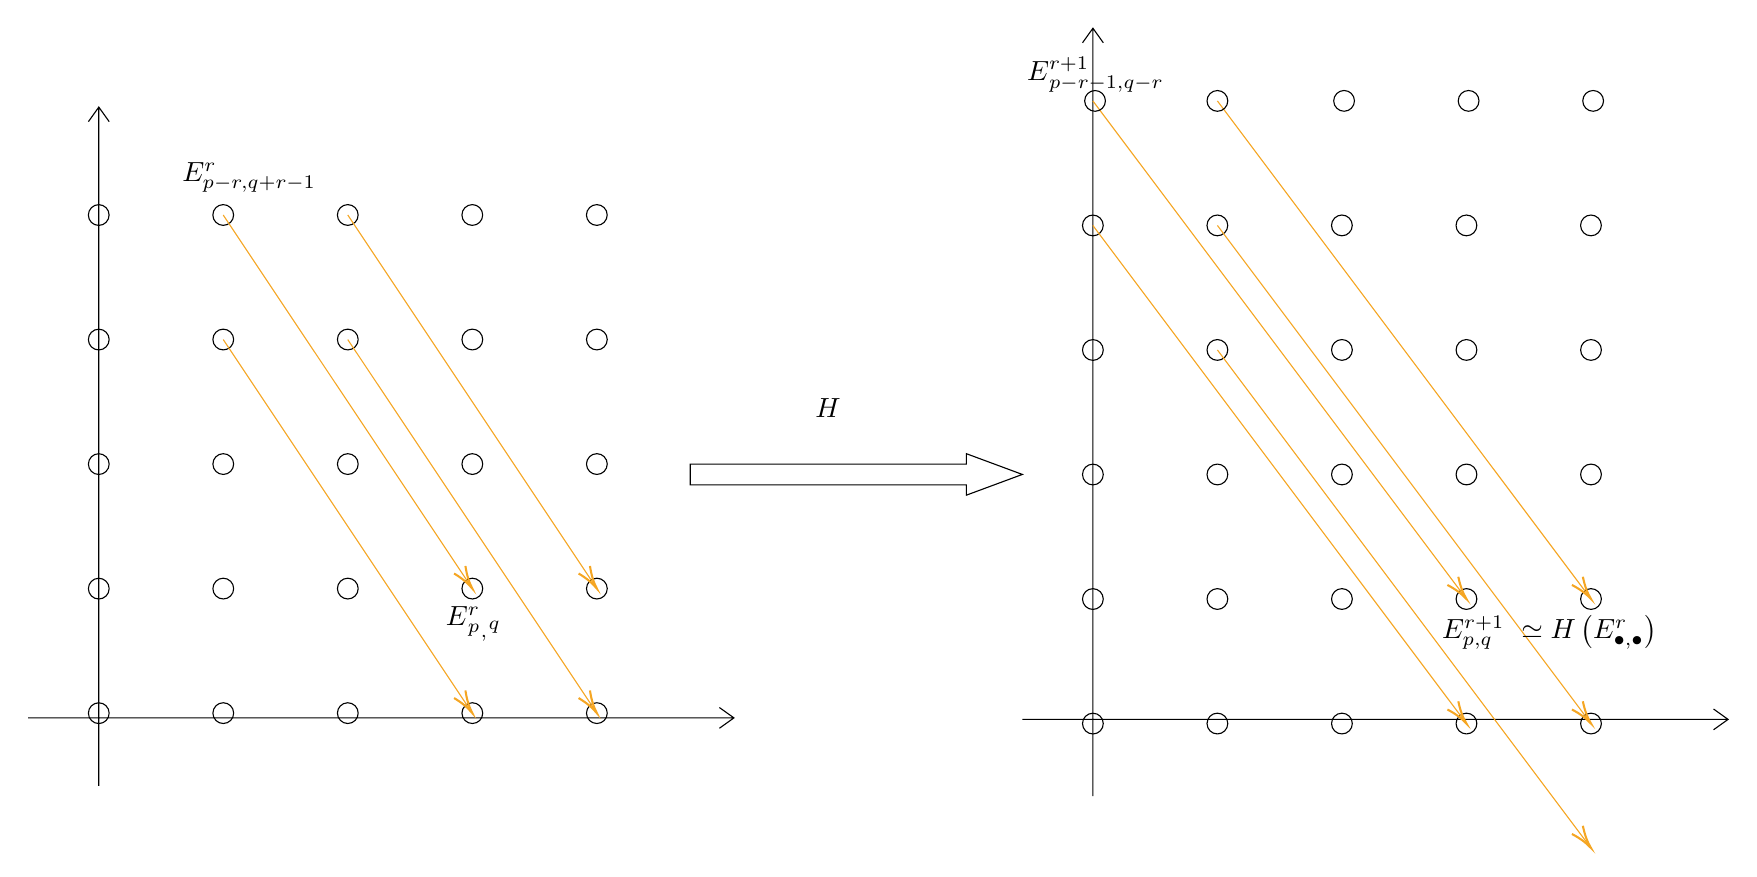
\begin{tikzpicture}[x=0.75pt,y=0.75pt,yscale=-1,xscale=1]
    %uncomment if require: \path (0,722); %set diagram left start at 0, and has height of 722
    
    %Shape: Circle [id:dp4266897237946641] 
    \draw   (75.02,105) .. controls (72.26,105.01) and (70.01,102.78) .. (70,100.02) .. controls (69.99,97.26) and (72.22,95.01) .. (74.98,95) .. controls (77.74,94.99) and (79.99,97.22) .. (80,99.98) .. controls (80.01,102.74) and (77.78,104.99) .. (75.02,105) -- cycle ;
    %Shape: Circle [id:dp21243284552909902] 
    \draw   (135,104.98) .. controls (132.24,104.99) and (129.99,102.76) .. (129.98,100) .. controls (129.97,97.24) and (132.2,94.99) .. (134.97,94.98) .. controls (137.73,94.97) and (139.97,97.2) .. (139.98,99.97) .. controls (139.99,102.73) and (137.76,104.97) .. (135,104.98) -- cycle ;
    %Shape: Circle [id:dp1121940024781991] 
    \draw   (195,104.98) .. controls (192.24,104.99) and (189.99,102.76) .. (189.98,100) .. controls (189.97,97.24) and (192.2,94.99) .. (194.97,94.98) .. controls (197.73,94.97) and (199.97,97.2) .. (199.98,99.97) .. controls (199.99,102.73) and (197.76,104.97) .. (195,104.98) -- cycle ;
    %Shape: Circle [id:dp03369431999743655] 
    \draw   (255,104.98) .. controls (252.24,104.99) and (249.99,102.76) .. (249.98,100) .. controls (249.97,97.24) and (252.2,94.99) .. (254.97,94.98) .. controls (257.73,94.97) and (259.97,97.2) .. (259.98,99.97) .. controls (259.99,102.73) and (257.76,104.97) .. (255,104.98) -- cycle ;
    %Shape: Circle [id:dp42374483173520405] 
    \draw   (315,104.98) .. controls (312.24,104.99) and (309.99,102.76) .. (309.98,100) .. controls (309.97,97.24) and (312.2,94.99) .. (314.97,94.98) .. controls (317.73,94.97) and (319.97,97.2) .. (319.98,99.97) .. controls (319.99,102.73) and (317.76,104.97) .. (315,104.98) -- cycle ;
    %Shape: Circle [id:dp929688933276159] 
    \draw   (75.03,165) .. controls (72.27,165.01) and (70.03,162.78) .. (70.02,160.02) .. controls (70.01,157.26) and (72.24,155.01) .. (75,155) .. controls (77.76,154.99) and (80.01,157.22) .. (80.02,159.98) .. controls (80.03,162.74) and (77.8,164.99) .. (75.03,165) -- cycle ;
    %Shape: Circle [id:dp06285342706484032] 
    \draw   (135.02,164.98) .. controls (132.26,164.99) and (130.01,162.76) .. (130,160) .. controls (129.99,157.24) and (132.22,154.99) .. (134.98,154.98) .. controls (137.74,154.97) and (139.99,157.2) .. (140,159.97) .. controls (140.01,162.73) and (137.78,164.97) .. (135.02,164.98) -- cycle ;
    %Shape: Circle [id:dp16743059497867363] 
    \draw   (195.02,164.98) .. controls (192.26,164.99) and (190.01,162.76) .. (190,160) .. controls (189.99,157.24) and (192.22,154.99) .. (194.98,154.98) .. controls (197.74,154.97) and (199.99,157.2) .. (200,159.97) .. controls (200.01,162.73) and (197.78,164.97) .. (195.02,164.98) -- cycle ;
    %Shape: Circle [id:dp36542937714360957] 
    \draw   (255.02,164.98) .. controls (252.26,164.99) and (250.01,162.76) .. (250,160) .. controls (249.99,157.24) and (252.22,154.99) .. (254.98,154.98) .. controls (257.74,154.97) and (259.99,157.2) .. (260,159.97) .. controls (260.01,162.73) and (257.78,164.97) .. (255.02,164.98) -- cycle ;
    %Shape: Circle [id:dp6038261663592559] 
    \draw   (315.02,164.98) .. controls (312.26,164.99) and (310.01,162.76) .. (310,160) .. controls (309.99,157.24) and (312.22,154.99) .. (314.98,154.98) .. controls (317.74,154.97) and (319.99,157.2) .. (320,159.97) .. controls (320.01,162.73) and (317.78,164.97) .. (315.02,164.98) -- cycle ;
    %Shape: Circle [id:dp6241943304358233] 
    \draw   (75.03,225) .. controls (72.27,225.01) and (70.03,222.78) .. (70.02,220.02) .. controls (70.01,217.26) and (72.24,215.01) .. (75,215) .. controls (77.76,214.99) and (80.01,217.22) .. (80.02,219.98) .. controls (80.03,222.74) and (77.8,224.99) .. (75.03,225) -- cycle ;
    %Shape: Circle [id:dp023236749364964338] 
    \draw   (135.02,224.98) .. controls (132.26,224.99) and (130.01,222.76) .. (130,220) .. controls (129.99,217.24) and (132.22,214.99) .. (134.98,214.98) .. controls (137.74,214.97) and (139.99,217.2) .. (140,219.97) .. controls (140.01,222.73) and (137.78,224.97) .. (135.02,224.98) -- cycle ;
    %Shape: Circle [id:dp36880988253650215] 
    \draw   (195.02,224.98) .. controls (192.26,224.99) and (190.01,222.76) .. (190,220) .. controls (189.99,217.24) and (192.22,214.99) .. (194.98,214.98) .. controls (197.74,214.97) and (199.99,217.2) .. (200,219.97) .. controls (200.01,222.73) and (197.78,224.97) .. (195.02,224.98) -- cycle ;
    %Shape: Circle [id:dp3351303968902207] 
    \draw   (255.02,224.98) .. controls (252.26,224.99) and (250.01,222.76) .. (250,220) .. controls (249.99,217.24) and (252.22,214.99) .. (254.98,214.98) .. controls (257.74,214.97) and (259.99,217.2) .. (260,219.97) .. controls (260.01,222.73) and (257.78,224.97) .. (255.02,224.98) -- cycle ;
    %Shape: Circle [id:dp4955586419456143] 
    \draw   (315.02,224.98) .. controls (312.26,224.99) and (310.01,222.76) .. (310,220) .. controls (309.99,217.24) and (312.22,214.99) .. (314.98,214.98) .. controls (317.74,214.97) and (319.99,217.2) .. (320,219.97) .. controls (320.01,222.73) and (317.78,224.97) .. (315.02,224.98) -- cycle ;
    %Shape: Circle [id:dp6522413670397201] 
    \draw   (75.03,285) .. controls (72.27,285.01) and (70.03,282.78) .. (70.02,280.02) .. controls (70.01,277.26) and (72.24,275.01) .. (75,275) .. controls (77.76,274.99) and (80.01,277.22) .. (80.02,279.98) .. controls (80.03,282.74) and (77.8,284.99) .. (75.03,285) -- cycle ;
    %Shape: Circle [id:dp35576468556246343] 
    \draw   (135.02,284.98) .. controls (132.26,284.99) and (130.01,282.76) .. (130,280) .. controls (129.99,277.24) and (132.22,274.99) .. (134.98,274.98) .. controls (137.74,274.97) and (139.99,277.2) .. (140,279.97) .. controls (140.01,282.73) and (137.78,284.97) .. (135.02,284.98) -- cycle ;
    %Shape: Circle [id:dp6007059503264247] 
    \draw   (195.02,284.98) .. controls (192.26,284.99) and (190.01,282.76) .. (190,280) .. controls (189.99,277.24) and (192.22,274.99) .. (194.98,274.98) .. controls (197.74,274.97) and (199.99,277.2) .. (200,279.97) .. controls (200.01,282.73) and (197.78,284.97) .. (195.02,284.98) -- cycle ;
    %Shape: Circle [id:dp37483501945609743] 
    \draw   (255.02,284.98) .. controls (252.26,284.99) and (250.01,282.76) .. (250,280) .. controls (249.99,277.24) and (252.22,274.99) .. (254.98,274.98) .. controls (257.74,274.97) and (259.99,277.2) .. (260,279.97) .. controls (260.01,282.73) and (257.78,284.97) .. (255.02,284.98) -- cycle ;
    %Shape: Circle [id:dp031933000616092166] 
    \draw   (315.02,284.98) .. controls (312.26,284.99) and (310.01,282.76) .. (310,280) .. controls (309.99,277.24) and (312.22,274.99) .. (314.98,274.98) .. controls (317.74,274.97) and (319.99,277.2) .. (320,279.97) .. controls (320.01,282.73) and (317.78,284.97) .. (315.02,284.98) -- cycle ;
    %Shape: Circle [id:dp6716130562985475] 
    \draw   (75.03,345) .. controls (72.27,345.01) and (70.03,342.78) .. (70.02,340.02) .. controls (70.01,337.26) and (72.24,335.01) .. (75,335) .. controls (77.76,334.99) and (80.01,337.22) .. (80.02,339.98) .. controls (80.03,342.74) and (77.8,344.99) .. (75.03,345) -- cycle ;
    %Shape: Circle [id:dp8715199531009215] 
    \draw   (135.02,344.98) .. controls (132.26,344.99) and (130.01,342.76) .. (130,340) .. controls (129.99,337.24) and (132.22,334.99) .. (134.98,334.98) .. controls (137.74,334.97) and (139.99,337.2) .. (140,339.97) .. controls (140.01,342.73) and (137.78,344.97) .. (135.02,344.98) -- cycle ;
    %Shape: Circle [id:dp173129730314039] 
    \draw   (195.02,344.98) .. controls (192.26,344.99) and (190.01,342.76) .. (190,340) .. controls (189.99,337.24) and (192.22,334.99) .. (194.98,334.98) .. controls (197.74,334.97) and (199.99,337.2) .. (200,339.97) .. controls (200.01,342.73) and (197.78,344.97) .. (195.02,344.98) -- cycle ;
    %Shape: Circle [id:dp009814893702278393] 
    \draw   (255.02,344.98) .. controls (252.26,344.99) and (250.01,342.76) .. (250,340) .. controls (249.99,337.24) and (252.22,334.99) .. (254.98,334.98) .. controls (257.74,334.97) and (259.99,337.2) .. (260,339.97) .. controls (260.01,342.73) and (257.78,344.97) .. (255.02,344.98) -- cycle ;
    %Shape: Circle [id:dp25088631700583985] 
    \draw   (315.02,344.98) .. controls (312.26,344.99) and (310.01,342.76) .. (310,340) .. controls (309.99,337.24) and (312.22,334.99) .. (314.98,334.98) .. controls (317.74,334.97) and (319.99,337.2) .. (320,339.97) .. controls (320.01,342.73) and (317.78,344.97) .. (315.02,344.98) -- cycle ;
    %Shape: Axis 2D [id:dp5312763907764603] 
    \draw  (41.03,342.28) -- (381.03,342.28)(75.03,48) -- (75.03,374.98) (374.03,337.28) -- (381.03,342.28) -- (374.03,347.28) (70.03,55) -- (75.03,48) -- (80.03,55)  ;
    %Shape: Circle [id:dp710928389895353] 
    \draw   (553.98,110.02) .. controls (551.22,110.03) and (548.97,107.8) .. (548.97,105.03) .. controls (548.96,102.27) and (551.19,100.03) .. (553.95,100.02) .. controls (556.71,100.01) and (558.96,102.24) .. (558.97,105) .. controls (558.97,107.76) and (556.74,110.01) .. (553.98,110.02) -- cycle ;
    %Shape: Circle [id:dp3176355719811016] 
    \draw   (613.97,110) .. controls (611.2,110.01) and (608.96,107.78) .. (608.95,105.02) .. controls (608.94,102.26) and (611.17,100.01) .. (613.93,100) .. controls (616.69,99.99) and (618.94,102.22) .. (618.95,104.98) .. controls (618.96,107.74) and (616.73,109.99) .. (613.97,110) -- cycle ;
    %Shape: Circle [id:dp3259866226783882] 
    \draw   (673.97,110) .. controls (671.2,110.01) and (668.96,107.78) .. (668.95,105.02) .. controls (668.94,102.26) and (671.17,100.01) .. (673.93,100) .. controls (676.69,99.99) and (678.94,102.22) .. (678.95,104.98) .. controls (678.96,107.74) and (676.73,109.99) .. (673.97,110) -- cycle ;
    %Shape: Circle [id:dp5147394211208863] 
    \draw   (733.97,110) .. controls (731.2,110.01) and (728.96,107.78) .. (728.95,105.02) .. controls (728.94,102.26) and (731.17,100.01) .. (733.93,100) .. controls (736.69,99.99) and (738.94,102.22) .. (738.95,104.98) .. controls (738.96,107.74) and (736.73,109.99) .. (733.97,110) -- cycle ;
    %Shape: Circle [id:dp23145851018270502] 
    \draw   (793.97,110) .. controls (791.2,110.01) and (788.96,107.78) .. (788.95,105.02) .. controls (788.94,102.26) and (791.17,100.01) .. (793.93,100) .. controls (796.69,99.99) and (798.94,102.22) .. (798.95,104.98) .. controls (798.96,107.74) and (796.73,109.99) .. (793.97,110) -- cycle ;
    %Shape: Circle [id:dp9375931907888719] 
    \draw   (554,170.02) .. controls (551.24,170.03) and (548.99,167.8) .. (548.98,165.03) .. controls (548.97,162.27) and (551.2,160.03) .. (553.97,160.02) .. controls (556.73,160.01) and (558.97,162.24) .. (558.98,165) .. controls (558.99,167.76) and (556.76,170.01) .. (554,170.02) -- cycle ;
    %Shape: Circle [id:dp02207041636329654] 
    \draw   (613.98,170) .. controls (611.22,170.01) and (608.97,167.78) .. (608.97,165.02) .. controls (608.96,162.26) and (611.19,160.01) .. (613.95,160) .. controls (616.71,159.99) and (618.96,162.22) .. (618.97,164.98) .. controls (618.97,167.74) and (616.74,169.99) .. (613.98,170) -- cycle ;
    %Shape: Circle [id:dp3467806733782305] 
    \draw   (673.98,170) .. controls (671.22,170.01) and (668.97,167.78) .. (668.97,165.02) .. controls (668.96,162.26) and (671.19,160.01) .. (673.95,160) .. controls (676.71,159.99) and (678.96,162.22) .. (678.97,164.98) .. controls (678.97,167.74) and (676.74,169.99) .. (673.98,170) -- cycle ;
    %Shape: Circle [id:dp14292807542315533] 
    \draw   (733.98,170) .. controls (731.22,170.01) and (728.97,167.78) .. (728.97,165.02) .. controls (728.96,162.26) and (731.19,160.01) .. (733.95,160) .. controls (736.71,159.99) and (738.96,162.22) .. (738.97,164.98) .. controls (738.97,167.74) and (736.74,169.99) .. (733.98,170) -- cycle ;
    %Shape: Circle [id:dp673487111283906] 
    \draw   (793.98,170) .. controls (791.22,170.01) and (788.97,167.78) .. (788.97,165.02) .. controls (788.96,162.26) and (791.19,160.01) .. (793.95,160) .. controls (796.71,159.99) and (798.96,162.22) .. (798.97,164.98) .. controls (798.97,167.74) and (796.74,169.99) .. (793.98,170) -- cycle ;
    %Shape: Circle [id:dp06416624559062312] 
    \draw   (554,230.02) .. controls (551.24,230.03) and (548.99,227.8) .. (548.98,225.03) .. controls (548.97,222.27) and (551.2,220.03) .. (553.97,220.02) .. controls (556.73,220.01) and (558.97,222.24) .. (558.98,225) .. controls (558.99,227.76) and (556.76,230.01) .. (554,230.02) -- cycle ;
    %Shape: Circle [id:dp6307300465695588] 
    \draw   (613.98,230) .. controls (611.22,230.01) and (608.97,227.78) .. (608.97,225.02) .. controls (608.96,222.26) and (611.19,220.01) .. (613.95,220) .. controls (616.71,219.99) and (618.96,222.22) .. (618.97,224.98) .. controls (618.97,227.74) and (616.74,229.99) .. (613.98,230) -- cycle ;
    %Shape: Circle [id:dp08524010691121786] 
    \draw   (673.98,230) .. controls (671.22,230.01) and (668.97,227.78) .. (668.97,225.02) .. controls (668.96,222.26) and (671.19,220.01) .. (673.95,220) .. controls (676.71,219.99) and (678.96,222.22) .. (678.97,224.98) .. controls (678.97,227.74) and (676.74,229.99) .. (673.98,230) -- cycle ;
    %Shape: Circle [id:dp5621602892375971] 
    \draw   (733.98,230) .. controls (731.22,230.01) and (728.97,227.78) .. (728.97,225.02) .. controls (728.96,222.26) and (731.19,220.01) .. (733.95,220) .. controls (736.71,219.99) and (738.96,222.22) .. (738.97,224.98) .. controls (738.97,227.74) and (736.74,229.99) .. (733.98,230) -- cycle ;
    %Shape: Circle [id:dp9353039279710524] 
    \draw   (793.98,230) .. controls (791.22,230.01) and (788.97,227.78) .. (788.97,225.02) .. controls (788.96,222.26) and (791.19,220.01) .. (793.95,220) .. controls (796.71,219.99) and (798.96,222.22) .. (798.97,224.98) .. controls (798.97,227.74) and (796.74,229.99) .. (793.98,230) -- cycle ;
    %Shape: Circle [id:dp5507320336575935] 
    \draw   (554,290.02) .. controls (551.24,290.03) and (548.99,287.8) .. (548.98,285.03) .. controls (548.97,282.27) and (551.2,280.03) .. (553.97,280.02) .. controls (556.73,280.01) and (558.97,282.24) .. (558.98,285) .. controls (558.99,287.76) and (556.76,290.01) .. (554,290.02) -- cycle ;
    %Shape: Circle [id:dp4523095042243699] 
    \draw   (613.98,290) .. controls (611.22,290.01) and (608.97,287.78) .. (608.97,285.02) .. controls (608.96,282.26) and (611.19,280.01) .. (613.95,280) .. controls (616.71,279.99) and (618.96,282.22) .. (618.97,284.98) .. controls (618.97,287.74) and (616.74,289.99) .. (613.98,290) -- cycle ;
    %Shape: Circle [id:dp06125859355644436] 
    \draw   (673.98,290) .. controls (671.22,290.01) and (668.97,287.78) .. (668.97,285.02) .. controls (668.96,282.26) and (671.19,280.01) .. (673.95,280) .. controls (676.71,279.99) and (678.96,282.22) .. (678.97,284.98) .. controls (678.97,287.74) and (676.74,289.99) .. (673.98,290) -- cycle ;
    %Shape: Circle [id:dp4815281940551307] 
    \draw   (733.98,290) .. controls (731.22,290.01) and (728.97,287.78) .. (728.97,285.02) .. controls (728.96,282.26) and (731.19,280.01) .. (733.95,280) .. controls (736.71,279.99) and (738.96,282.22) .. (738.97,284.98) .. controls (738.97,287.74) and (736.74,289.99) .. (733.98,290) -- cycle ;
    %Shape: Circle [id:dp7856072243294682] 
    \draw   (793.98,290) .. controls (791.22,290.01) and (788.97,287.78) .. (788.97,285.02) .. controls (788.96,282.26) and (791.19,280.01) .. (793.95,280) .. controls (796.71,279.99) and (798.96,282.22) .. (798.97,284.98) .. controls (798.97,287.74) and (796.74,289.99) .. (793.98,290) -- cycle ;
    %Shape: Circle [id:dp8154588161590131] 
    \draw   (554,350.02) .. controls (551.24,350.03) and (548.99,347.8) .. (548.98,345.03) .. controls (548.97,342.27) and (551.2,340.03) .. (553.97,340.02) .. controls (556.73,340.01) and (558.97,342.24) .. (558.98,345) .. controls (558.99,347.76) and (556.76,350.01) .. (554,350.02) -- cycle ;
    %Shape: Circle [id:dp10771086552348696] 
    \draw   (613.98,350) .. controls (611.22,350.01) and (608.97,347.78) .. (608.97,345.02) .. controls (608.96,342.26) and (611.19,340.01) .. (613.95,340) .. controls (616.71,339.99) and (618.96,342.22) .. (618.97,344.98) .. controls (618.97,347.74) and (616.74,349.99) .. (613.98,350) -- cycle ;
    %Shape: Circle [id:dp23425510172154118] 
    \draw   (673.98,350) .. controls (671.22,350.01) and (668.97,347.78) .. (668.97,345.02) .. controls (668.96,342.26) and (671.19,340.01) .. (673.95,340) .. controls (676.71,339.99) and (678.96,342.22) .. (678.97,344.98) .. controls (678.97,347.74) and (676.74,349.99) .. (673.98,350) -- cycle ;
    %Shape: Circle [id:dp8278159849860861] 
    \draw   (733.98,350) .. controls (731.22,350.01) and (728.97,347.78) .. (728.97,345.02) .. controls (728.96,342.26) and (731.19,340.01) .. (733.95,340) .. controls (736.71,339.99) and (738.96,342.22) .. (738.97,344.98) .. controls (738.97,347.74) and (736.74,349.99) .. (733.98,350) -- cycle ;
    %Shape: Circle [id:dp8853027091802028] 
    \draw   (793.98,350) .. controls (791.22,350.01) and (788.97,347.78) .. (788.97,345.02) .. controls (788.96,342.26) and (791.19,340.01) .. (793.95,340) .. controls (796.71,339.99) and (798.96,342.22) .. (798.97,344.98) .. controls (798.97,347.74) and (796.74,349.99) .. (793.98,350) -- cycle ;
    %Shape: Axis 2D [id:dp6032520025857421] 
    \draw  (520,343) -- (860,343)(554,10) -- (554,380) (853,338) -- (860,343) -- (853,348) (549,17) -- (554,10) -- (559,17)  ;
    %Straight Lines [id:da785524365210303] 
    \draw [color={rgb, 255:red, 245; green, 166; blue, 35 }  ,draw opacity=1 ]   (134.98,99.98) -- (253.89,278.32) ;
    \draw [shift={(255,279.98)}, rotate = 236.31] [color={rgb, 255:red, 245; green, 166; blue, 35 }  ,draw opacity=1 ][line width=0.75]    (10.93,-3.29) .. controls (6.95,-1.4) and (3.31,-0.3) .. (0,0) .. controls (3.31,0.3) and (6.95,1.4) .. (10.93,3.29)   ;
    %Straight Lines [id:da6690802767816856] 
    \draw [color={rgb, 255:red, 245; green, 166; blue, 35 }  ,draw opacity=1 ]   (134.98,159.98) -- (253.89,338.32) ;
    \draw [shift={(255,339.98)}, rotate = 236.31] [color={rgb, 255:red, 245; green, 166; blue, 35 }  ,draw opacity=1 ][line width=0.75]    (10.93,-3.29) .. controls (6.95,-1.4) and (3.31,-0.3) .. (0,0) .. controls (3.31,0.3) and (6.95,1.4) .. (10.93,3.29)   ;
    %Straight Lines [id:da8728335334812608] 
    \draw [color={rgb, 255:red, 245; green, 166; blue, 35 }  ,draw opacity=1 ]   (194.98,159.98) -- (313.89,338.32) ;
    \draw [shift={(315,339.98)}, rotate = 236.31] [color={rgb, 255:red, 245; green, 166; blue, 35 }  ,draw opacity=1 ][line width=0.75]    (10.93,-3.29) .. controls (6.95,-1.4) and (3.31,-0.3) .. (0,0) .. controls (3.31,0.3) and (6.95,1.4) .. (10.93,3.29)   ;
    %Straight Lines [id:da35483773693673626] 
    \draw [color={rgb, 255:red, 245; green, 166; blue, 35 }  ,draw opacity=1 ]   (194.98,99.98) -- (313.89,278.32) ;
    \draw [shift={(315,279.98)}, rotate = 236.31] [color={rgb, 255:red, 245; green, 166; blue, 35 }  ,draw opacity=1 ][line width=0.75]    (10.93,-3.29) .. controls (6.95,-1.4) and (3.31,-0.3) .. (0,0) .. controls (3.31,0.3) and (6.95,1.4) .. (10.93,3.29)   ;
    %Straight Lines [id:da12487629487109653] 
    \draw [color={rgb, 255:red, 245; green, 166; blue, 35 }  ,draw opacity=1 ]   (553.97,45.02) -- (732.77,283.4) ;
    \draw [shift={(733.97,285)}, rotate = 233.13] [color={rgb, 255:red, 245; green, 166; blue, 35 }  ,draw opacity=1 ][line width=0.75]    (10.93,-3.29) .. controls (6.95,-1.4) and (3.31,-0.3) .. (0,0) .. controls (3.31,0.3) and (6.95,1.4) .. (10.93,3.29)   ;
    %Shape: Circle [id:dp6992072206020716] 
    \draw   (555.03,50.02) .. controls (552.27,50.03) and (550.03,47.8) .. (550.02,45.03) .. controls (550.01,42.27) and (552.24,40.03) .. (555,40.02) .. controls (557.76,40.01) and (560.01,42.24) .. (560.02,45) .. controls (560.03,47.76) and (557.8,50.01) .. (555.03,50.02) -- cycle ;
    %Straight Lines [id:da8466985373644896] 
    \draw [color={rgb, 255:red, 245; green, 166; blue, 35 }  ,draw opacity=1 ]   (553.97,105.02) -- (732.77,343.4) ;
    \draw [shift={(733.97,345)}, rotate = 233.13] [color={rgb, 255:red, 245; green, 166; blue, 35 }  ,draw opacity=1 ][line width=0.75]    (10.93,-3.29) .. controls (6.95,-1.4) and (3.31,-0.3) .. (0,0) .. controls (3.31,0.3) and (6.95,1.4) .. (10.93,3.29)   ;
    %Straight Lines [id:da8657860948269241] 
    \draw [color={rgb, 255:red, 245; green, 166; blue, 35 }  ,draw opacity=1 ]   (613.97,165) -- (792.77,403.38) ;
    \draw [shift={(793.97,404.98)}, rotate = 233.13] [color={rgb, 255:red, 245; green, 166; blue, 35 }  ,draw opacity=1 ][line width=0.75]    (10.93,-3.29) .. controls (6.95,-1.4) and (3.31,-0.3) .. (0,0) .. controls (3.31,0.3) and (6.95,1.4) .. (10.93,3.29)   ;
    %Straight Lines [id:da6057260631851047] 
    \draw [color={rgb, 255:red, 245; green, 166; blue, 35 }  ,draw opacity=1 ]   (613.97,45.02) -- (792.77,283.4) ;
    \draw [shift={(793.97,285)}, rotate = 233.13] [color={rgb, 255:red, 245; green, 166; blue, 35 }  ,draw opacity=1 ][line width=0.75]    (10.93,-3.29) .. controls (6.95,-1.4) and (3.31,-0.3) .. (0,0) .. controls (3.31,0.3) and (6.95,1.4) .. (10.93,3.29)   ;
    %Shape: Circle [id:dp13215988211910135] 
    \draw   (613.98,50.02) .. controls (611.22,50.03) and (608.97,47.8) .. (608.97,45.03) .. controls (608.96,42.27) and (611.19,40.03) .. (613.95,40.02) .. controls (616.71,40.01) and (618.96,42.24) .. (618.97,45) .. controls (618.97,47.76) and (616.74,50.01) .. (613.98,50.02) -- cycle ;
    %Shape: Circle [id:dp024155588166657527] 
    \draw   (675.02,50) .. controls (672.26,50.01) and (670.01,47.78) .. (670,45.02) .. controls (669.99,42.26) and (672.22,40.01) .. (674.98,40) .. controls (677.74,39.99) and (679.99,42.22) .. (680,44.98) .. controls (680.01,47.74) and (677.78,49.99) .. (675.02,50) -- cycle ;
    %Shape: Circle [id:dp32371319961886247] 
    \draw   (735.02,50) .. controls (732.26,50.01) and (730.01,47.78) .. (730,45.02) .. controls (729.99,42.26) and (732.22,40.01) .. (734.98,40) .. controls (737.74,39.99) and (739.99,42.22) .. (740,44.98) .. controls (740.01,47.74) and (737.78,49.99) .. (735.02,50) -- cycle ;
    %Shape: Circle [id:dp08187917829768343] 
    \draw   (795.02,50) .. controls (792.26,50.01) and (790.01,47.78) .. (790,45.02) .. controls (789.99,42.26) and (792.22,40.01) .. (794.98,40) .. controls (797.74,39.99) and (799.99,42.22) .. (800,44.98) .. controls (800.01,47.74) and (797.78,49.99) .. (795.02,50) -- cycle ;
    %Straight Lines [id:da6068589813776775] 
    \draw [color={rgb, 255:red, 245; green, 166; blue, 35 }  ,draw opacity=1 ]   (613.97,105.02) -- (792.77,343.4) ;
    \draw [shift={(793.97,345)}, rotate = 233.13] [color={rgb, 255:red, 245; green, 166; blue, 35 }  ,draw opacity=1 ][line width=0.75]    (10.93,-3.29) .. controls (6.95,-1.4) and (3.31,-0.3) .. (0,0) .. controls (3.31,0.3) and (6.95,1.4) .. (10.93,3.29)   ;
    %Right Arrow [id:dp32527154048889395] 
    \draw   (360,219.98) -- (493,219.98) -- (493,214.98) -- (520,224.98) -- (493,234.98) -- (493,229.98) -- (360,229.98) -- cycle ;
    
    
    % Text Node
    \draw (241,287.38) node [anchor=north west][inner sep=0.75pt]    {$E{_{p}^{r}}_{,}{}_{q}$};
    % Text Node
    \draw (114,73.38) node [anchor=north west][inner sep=0.75pt]    {$E_{p-r,q+r-1}^{r}$};
    % Text Node
    \draw (721,291.4) node [anchor=north west][inner sep=0.75pt]    {$E_{p,q}^{r+1} \ \simeq H\left( E_{\bullet ,\bullet }^{r}\right) \ $};
    % Text Node
    \draw (521,22.4) node [anchor=north west][inner sep=0.75pt]    {$E{_{p-r-1,q-r}^{r+1}}{}$};
    % Text Node
    \draw (419,187.38) node [anchor=north west][inner sep=0.75pt]    {$H$};
    
    
    \end{tikzpicture}
    \end{figure}
    

%There is a \textbf{category of homology spectral sequences}; a morphism $f: E^{\prime} \rightarrow$ $E$ is a family of maps $f_{p q}^r: E_{p q}^{\prime} \rightarrow E_{p q}^r$ in $\mathcal{A}$ (for $r$ suitably large) with $d^r f^r=$ $f^r d^r$ such that each $f_{p q}^{r+1}$ is the map induced by $f_{p q}^r$ on homology.

\subsubsection{Bounded convergence}

A homology spectral sequence is said to be \textbf{bounded} if for each $n$ there are only finitely many nonzero terms of total degree $n$ in $E_{* *}^a$. If so, then for each $p$ and $q$ there is an $r_0$ such that $E_{p q}^r=$ $E_{p q}^{r+1}$ for all $r \geq r_0$. We write $E_{p q}^{\infty}$ for this stable value of $E_{p q}^r$.\\
To see this, consider a first quadrant spectral sequence $E^a _{pq}$. If we fix $p$ and $q$, then $E_{p q}^r=E_{p q}^{r+1}$ for all large $r(r>\max \{p, q+1\}$ will do), because the $d^r$ landing in the ( $p, q$ ) spot come from the fourth quadrant, while the $d^r$ leaving $E_{p q}^r$ land in the second quadrant.\\ 

We say that a bounded spectral sequence \textbf{converges} to $H_*$ if we are given a family of objects $H_n$ of $\mathcal{A}$, each having a finite filtration
$$
0=F_s H_n \subseteq \cdots \subseteq F_{p-1} H_n \subseteq F_p H_n \subseteq F_{p+1} H_n \subseteq \cdots \subseteq F_t H_n=H_n,
$$
and we are given isomorphisms $E_{p q}^{\infty} \cong F_p H_{p+q} / F_{p-1} H_{p+q}$. The traditional symbolic way of describing such a bounded convergence is like this:
$$
E_{p q}^a \Rightarrow H_{p+q}
$$

A (homology) spectral sequence \textbf{collapses at $E^r(r \geq 1)$ } if there is exactly one nonzero row or column in the lattice $\left\{E_{p q}^r\right\}$.\\
If a collapsing spectral sequence converges to $H_*$, we can read the $H_n$ off: $H_n$ is the unique nonzero $E_{p q}^r$ with $p+q=n$. The overwhelming majority of all applications of spectral sequences involve spectral sequences that collapse at $E^1$ or $E^2$.\\
%mapping cone and spectral sequences exercise 5.4.4!!

You could stop after reading this part! Just take a look on the Lerray-Serre spectral sequence.\\


\subsubsection{General case}

We are assuming axioms (Ab4) and (Ab4$^*$)!\\

Given a homology spectral sequence, we see that each $E_{p q}^{r+1}$ is a subquotient of the previous term $E_{p q}^r$. By induction on $r$, we see that there is a nested family of subobjects of $E_{p q}^a$ :
$$
0=B_{p q}^a \subseteq \cdots \subseteq B_{p q}^r \subseteq B_{p q}^{r+1} \subseteq \cdots \subseteq Z_{p q}^{r+1} \subseteq Z_{p q}^r \subseteq \cdots \subseteq Z_{p q}^a=E_{p q}^a
$$
such that $E_{p q}^r \cong Z_{p q}^r / B_{p q}^r$. We introduce the intermediate objects
$$
B_{p q}^{\infty}=\bigcup_{r=a}^{\infty} B_{p q}^r \quad \text { and } \quad Z_{p q}^{\infty}=\bigcap_{r=a}^{\infty} Z_{p q}^r
$$
and define $E_{p q}^{\infty}=Z_{p q}^{\infty} / B_{p q}^{\infty}$. In a bounded spectral sequence both the union and intersection are finite, so $B_{p q}^{\infty}=B_{p q}^r$ and $Z_{p q}^{\infty}=Z_{p q}^r$ for large $r$. Thus this definition agrees with the previous one.\\
A homology spectral sequence is said to be \textbf{bounded below }if for each $n$ there is an integer $s=s(n)$ such that the terms $E_{p q}^a$ of total degree $n$ vanish for all $p<s$. These spectral sequences have good convergence properties. Bounded spectral sequences are bounded below. Right half-plane homology spectral sequences are bounded below but not bounded.\\

We say the spectral sequence \textbf{weakly converges} to $H_*$ if we are given objects $H_n$ of $\mathcal{A}$, each having a filtration
$$
\cdots \subseteq F_{p-1} H_n \subseteq F_p H_n \subseteq F_{p+1} H_n \subseteq \cdots \subseteq H_n,
$$
together with isomorphisms $\beta_{p q}: E_{p q}^{\infty} \cong F_p H_{p+q} / F_{p-1} H_{p+q}$ for all $p$ and $q$. Note that a weakly convergent spectral sequence cannot detect elements of $\cap F_p H_n$, nor can it detect elements in $H_n$ that are not in $\cup F_p H_n$.\\
We say that the spectral sequence $\left\{E_{p q}^r\right\}$ approaches $H_*$ (or \textbf{abuts} to $H_*$ ) if it weakly converges to $H_*$ and we also have $H_n=\cup F_p H_n$ and $\cap F_p H_n=0$ for all $n$. Every weakly convergent spectral sequence approaches $\cup F_p H_* / \cap$ $F_p H_*$.\\

We say that a spectral sequence is \textbf{regular} if for each $p$ and $q$ the differentials $d_{p q}^r$ (or $d_r^{p q}$ ) leaving $E_{p q}^r$ (or $E_r^{p q}$ ) are zero for all large $r$. \\
Regularity is the most useful general condition for convergence used in practice; bounded below spectral sequences are also regular. Note that a spectral sequence is regular iff for each $p$ and $q: Z_{p q}^{\infty}=Z_{p q}^r$ for all large $r$.\\

We say that the spectral sequence \textbf{converges} to $H_*$ if it approaches $H_*$, it is regular, and $H_n=\lim \left(H_n / F_p H_n\right)$ for each $n$.\\ 
A bounded below spectral sequence converges to $H_*$ whenever it approaches $H_*$, because the inverse limit condition is always satisfied in a bounded below spectral sequence.\\
We say that a map $h: H_* \rightarrow H_*^{\prime}$ is compatible with a morphism $f: E \rightarrow E^{\prime}$ if $h$ maps $F_p H_n$ to $F_p H_n^{\prime}$ and the associated maps $F_p H_n / F_{p-1} H_n \rightarrow F_p H_n^{\prime} / F_{p-1} H_n^{\prime}$ correspond under $\beta$ and $\beta^{\prime}$ to $f_{p q}^{\infty}: E_{p q}^{\infty} \rightarrow$ $E_{p q}^{\prime} \quad(q=n-p)$

\begin{theo}[Comparison Theorem]
Let $\left\{E_{p q}^r\right\}$ and $\left\{E_{p q}^{\prime r}\right\}$ converge to $H_*$ and $H_*^{\prime}$, respectively. Suppose given a map $h: H_* \rightarrow H_*^{\prime}$ compatible with a morphism $f: E \rightarrow E^{\prime}$ of spectral sequences. If $f^r: E_{p q}^r \cong E_{p q}^{\prime r}$ is an isomorphism for all $p$ and $q$ and some $r$ (hence for $r=\infty$ by the Mapping Lemma), then $h: H_* \rightarrow H_*^{\prime}$ is an isomorphism. 
\end{theo}

\subsubsection*{Filtered Chains}
A filtration $F$ on a chain complex $C$ is an ordered family of chain subcomplexes $\cdots \subseteq F_{p-1} C \subseteq F_p C \subseteq \cdots$ of $C$. The filtration is \textbf{exhaustive} if $C=\cup F_p C$. \\
A filtration on a chain complex $C$ is called \textbf{bounded} if for each $n$ there are integers $s<t$ such that $F_s C_n=0$ and $F_t C_n=C_n$. In this case, there are only finitely many nonzero terms of total degree $n$ in $E_{* *}^0$, so the spectral sequence is bounded.\\
The filtration is called \textbf{bounded below} if for each $n$ there is an integer $s$ so that $F_s C_n=0$, and it is called \textbf{bounded above} if for each $n$ there is a $t$ so that $F_t C_n=C_n$. Bounded filtrations are bounded above and below. Being bounded above is merely an easy way to ensure that a filtration is exhaustive. %are these definitions equivalent?

\begin{example}
We call the filtration \textbf{canonically bounded} if $F_{-1} C=0$ and $F_n C_n=C_n$ for each $n$. As $E_{p q}^0=$ $F_p C_{p+q} / F_{p-1} C_{p+q}$, every canonically bounded filtration gives rise to a first quadrant spectral sequence (converging to $H_*(C)$ ). For example, the Leray- Serre spectral sequence arises from a canonically bounded filtration of the singular chain complex $S_*(E)$. %ver geometria
\end{example}

\begin{theo}[Construction of a spectral sequence]
A filtration $F$ of a chain complex $C$ naturally determines a spectral sequence starting with $E_{p q}^0=F_p C_{p+q} / F_{p-1} C_{p+q}$ and $E_{p q}^1=H_{p+q}\left(E_{p *}^0\right)$.    
\end{theo}

A filtration on a chain complex $C$ is called \textbf{Hausdorff} if $\cap F_p C=0$. It will be clear from the construction that both $C$ and its Hausdorff quotient $C^h=C / \cap F_p C$ give rise to the same spectral sequence.\\
A filtration on $C$ is called \textbf{complete} if $C=\lim C / F_p C$. Complete filtrations are Hausdorff because $\cap F_p C$ is the kernel of the map from $C$ to its completion $\widehat{C}=\operatorname{\operatorname {lim}} C / F_p C$ (which is also a filtered complex: $F_n \widehat{C}=$ $\left.\underset{\longleftarrow}{\lim } F_n C / F_p C\right)$. \\
Bounded below filtrations are complete, and hence Hausdorff, because $F_s H_n(C)=0$ for each $n$.

\begin{coro}
The two spectral sequences arising from $C$ and $\widehat{C}$ are the same.    
\end{coro}

A filtration on a chain complex $C$ induces a filtration on the homology of $C: F_p H_n(C)$ is the image of the map $H_n\left(F_p C\right) \rightarrow H_n(C)$. If the filtration on $C$ is exhaustive, then the filtration on $H_n$ is also exhaustive $\left(H_n=\cup F_p H_n\right)$, because every element of $H_n$ is represented by an element $c$ of some $F_p C_n$ such that $d(c)=0$. If the filtration on $C$ is bounded below then the filtration on each $H_n(C)$ is also bounded below, since $F_p C=0$ implies that $F_p H_n(C)=0$. But this not happen with Hausdorff condition.

\begin{theo}[Classical convergence]
\begin{enumerate}
    \item Suppose that the filtration on $C$ is bounded. Then the spectral sequence is bounded and converges to $H_*(C)$ :
    $$
    E_{p q}^1=H_{p+q}\left(F_p C / F_{p-1} C\right) \Rightarrow H_{p+q}(C) .
    $$
    \item Suppose that the filtration on $C$ is bounded below and exhaustive. Then the spectral sequence is bounded below and also converges to $H_*(C)$.
    Moreover, the convergence is natural in the sense that if $f: C \rightarrow C^{\prime}$ is a map of filtered complexes, then the map $f_*: H_*(C) \rightarrow H_*\left(C^{\prime}\right)$ is compatible with the corresponding map of spectral sequences.
\end{enumerate}   
\end{theo}



\begin{theo}[Complete convergence]
Suppose that the filtration on $C$ is complete and exhaustive and the spectral sequence is regular (5.2.10). Then:
\begin{enumerate}
    \item 1. The spectral sequence weakly converges to $H_*(C)$.
    \item If the spectral sequence is bounded above, it converges to $H_*(C)$.
\end{enumerate}
\end{theo}

\subsection{Spectral sequences from double complexes}
There are two filtrations associated to every double complex $C$ (seen as a complex of complexes), resulting in two spectral sequences related to the homology of $\operatorname{Tot}(C)$, each one with interesting properties. The interplay between them is the key of many calculations.\\ %seria bueno definir filtered objects in general??


\textbf{Filtration by columns.} If $C=C_{* *}$ is a double complex, we may filter the (product or direct sum) total complex $\operatorname{Tot}(C)$ by the columns of $C$, letting ${ }^I F_n \operatorname{Tot}(C)$ be the total complex of the double subcomplex $\left({ }^I \tau_{\leq n} C\right)_{p q}= \begin{cases}C_{p q} & \text { if } p \leq n \\ 0 & \text { if } p>n\end{cases}$ of $C$. This gives rise to a spectral sequence $\left\{{ }^I E_{p q}^r\right\}$, starting with ${ }^I E_{p q}^0=C_{p q}$. The maps $d^0$ are just the vertical differentials $d^v$ of $C$, so
$$
{ }^I E_{p q}^1=H_q^v\left(C_{p *}\right)
$$

The maps $d^1: H_q^v\left(C_{p *}\right) \rightarrow H_q^v\left(C_{p-1, *}\right)$ are induced on homology from the horizontal differentials $d^h$ of $C$, so we may use the suggestive notation:
$$
{}^I E_{p q}^2=H_p^h H_q^v(C)
$$

If $C$ is a first quadrant double complex, the filtration is canonically bounded, and we have the convergent spectral sequence as in the previous section:
$$
{ }^I E_{p q}^2=H_p^h H_q^v(C) \Rightarrow H_{p+q}(\operatorname{Tot}(C))
$$

\textbf{Filtration by rows.} If $C$ is a double complex, we may also filter $\operatorname{Tot}(C)$ by the rows of $C$, letting ${ }^{I I} F_n \operatorname{Tot}(C)$ be the total complex of $\left({ }^{I I} \tau_{\leq n} C\right)_{p q}= \begin{cases}C_{p q} & \text { if } q \leq n \\ 0 & \text { if } q>n\end{cases}$. \\
Since $F_p \operatorname{Tot}(C) / F_{p-1} \operatorname{Tot}(C)$ is the row $C_{* p},{ }^I E_{p q}^0=C_{q p}$ and ${ }^{I I} E_{p q}^1=$ $H_q^h\left(C_{* p}\right)$. (Beware the interchange of $p$ and $q$ in the notation!) The maps $d^1$ are induced from the vertical differentials $d^v$ of $C$, so we may use the suggestive notation $$ {}^{II} E^2_{pq} = H^v _p H^h _q (C) .$$
Of course, this should not be surprising, since interchanging the roles of $p$ and $q$ converts the filtration by rows into the filtration by columns, and interchanges the spectral sequences ${ }^I E$ and ${ }^{I 1} E$.

As before, if $C$ is a first quadrant double complex, this filtration is canonically bounded, and the spectral sequence converges to $H_* \operatorname{Tot}(C)$.\\

We can prove the balancing property of Tor using both spectral sequences. We can also prove the Künneth formula, the Univeral Coefficient Theorem and the Acyclic Assembly Lemma from the following result:

\begin{theo}[Künneth spectral sequence]
Let $P$ be a bounded below complex of flat $R$-modules and $M$ an $R$-module. Then there is a boundedly converging right half-plane spectral sequence
    $$
    E_{p q}^2=\operatorname{Tor}_p^R\left(H_q(P), M\right) \Rightarrow H_{p+q}\left(P \otimes_R M\right)
    $$    
\end{theo}

\subsubsection{Hypercohomology}
Let $\mathcal{A}$ be an abelian category that has enough projectives. A\textbf{ (left) Cartan-Eilenberg resolution} $P_{* *}$ of a chain complex $A_*$ in $\mathcal{A}$ is an upper half-plane double complex ( $P_{p q}=0$ if $q<0$ ), consisting of projective objects of $\mathcal{A}$, together with a chain map ("augmentation") $P_{* 0} \xrightarrow{\epsilon} A_*$ such that for every $p$
\begin{enumerate}
    \item If $A_p=0$, the column $P_{p *}$ is zero.
    \item The maps on boundaries and homology
    $$
    \begin{aligned}
    & B_p(\epsilon): B_p\left(P, d^h\right) \rightarrow B_p(A) \\
    & H_p(\epsilon): H_p\left(P, d^h\right) \rightarrow H_p(A)
    \end{aligned}
    $$
    are projective resolutions in $\mathcal{A}$. Here $B_p\left(P, d^h\right)$ denotes the horizontal boundaries in the $(p, q)$ spot, that is, the chain complex whose $q^{t h}$ term is $d^h\left(P_{p+1, q}\right)$. The chain complexes $Z_p\left(P, d^h\right)$ and $H_p\left(P, d^h\right)=$ $Z_p\left(P, d^h\right) / B_p\left(P, d^h\right)$ are defined similarly.
\end{enumerate}

\begin{lemm}
    Every chain complex has a Cartan-Eilenberg resolution.
\end{lemm}

Let $f, g: D \rightarrow E$ be two maps of double complexes. A \textbf{chain homotopy} from $f$ to $g$ consists of maps $s_{p q}^h: D_{p q} \rightarrow E_{p+1, q}$ and $s_{p q}^v$ : $D_{p q} \rightarrow E_{p, q+1}$ so that
\[
g-f = (d^h s^h + s^h d^h) + (d^v s^v + s^v d^v)
\]
\[
s^v d^h+d^h s^v=s^h d^v+d^v s^h=0.
\]

This definition is set up so that $\left\{s^h+s^v\right.$ : $\left.\operatorname{Tot}(D)_n \rightarrow \operatorname{Tot}(E)_{n+1}\right\}$ forms an ordinary chain homotopy between the maps $\operatorname{Tot}(f)$ and $\operatorname{Tot}(g)$ from $\operatorname{Tot}^{\oplus}(D)$ to $\operatorname{Tot}^{\oplus}(E)$.

\begin{prop}
    \begin{enumerate}
        \item If $f, g: A \rightarrow B$ are homotopic maps of chain complexes, and $\tilde{f}, \tilde{g}: P \rightarrow$ $Q$ are maps of Cartan-Eilenberg resolutions lying over them, show that $\tilde{f}$ is chain homotopic to $\tilde{g}$.
        \item Show that any two Cartan-Eilenberg resolutions $P, Q$ of $A$ are chain homotopy equivalent. Conclude that for any additive functor $F$ the chain complexes $\operatorname{Tot}^{\oplus}(F(P))$ and $\operatorname{Tot}^{\oplus}(F(Q))$ are chain homotopy equivalent.
    \end{enumerate}
\end{prop}


Let $F: \mathcal{A} \rightarrow \mathcal{B}$ be a right exact functor, and assume that $\mathcal{A}$ has enough projectives. If $A$ is a chain complex in $\mathcal{A}$ and $P \rightarrow A$ is a Cartan-Eilenberg resolution, define $\mathbb{L}_i F(A)$ to be $H_i \operatorname{Tot}^{\oplus}(F(P))$. The Proposition shows that $\mathbb{L}_i F(A)$ is independent of the choice of $P$.\\
If $f: A \rightarrow B$ is a chain map and $\tilde{f}: P \rightarrow Q$ is a map of Cartan-Eilenberg resolutions over $f$, define $\mathbb{L}_i F(f)$ to be the map $H_i(\operatorname{Tot}(\tilde{f}))$ from $\mathbb{L}_i F(A)$ to $\mathbb{L}_i F(B)$. The Proposition implies that $\mathbb{L}_i F$ is a functor from $\operatorname{Ch}(\mathcal{A})$ to $\mathcal{B}$, at least when $\mathcal{B}$ is cocomplete. The $\mathbb{L}_i F$ are called the left hyper-derived functors of $F$.\\
If $\mathcal{B}$ is not cocomplete, $\operatorname{Tot}^{\oplus}(F(P))$ and $\mathbb{L}_i F(A)$ may not exist for all chain complexes $A$. In this case we restrict to the category $\mathrm{Ch}_{+}(\mathcal{A})$ of all chain complexes $A$ which are bounded below in the sense that there is a $p_0$ such that $A_p=0$ for $p<p_0$. Since $P_{p q}=0$ if $p<p_0$ or $q<0, \operatorname{Tot}^{\oplus}(F(P))$ exists in $\mathbf{C h}(\mathcal{B})$ and we may consider $\mathbb{L}_i F$ to be a functor from $\mathrm{Ch}_{+}(\mathcal{A})$ to $\mathcal{B}$.

\begin{lemm}
If $0 \rightarrow A \rightarrow B \rightarrow C \rightarrow 0$ is a short exact sequence of bounded below complexes, there is a long exact sequence
    $$
    \cdots \mathbb{L}_{i+1} F(C) \xrightarrow{\delta} \mathbb{L}_i F(A) \rightarrow \mathbb{L}_i F(B) \rightarrow \mathbb{L}_i F(C) \xrightarrow{\delta} \cdots
    $$    
\end{lemm}


\begin{prop}
There is always a convergent spectral sequence
    $$
    { }^{I I} E_{p q}^2=\left(L_p F\right)\left(H_q(A)\right) \Rightarrow \mathbb{L}_{p+q} F(A) .
    $$
    
    If $A$ is bounded below, there is a convergent spectral sequence
    $$
    { }^I E_{p q}^2=H_p\left(L_q F(A)\right) \Rightarrow \mathbb{L}_{p+q} F(A)
    $$   
\end{prop}

\begin{coro}
\begin{enumerate}
    \item If $A$ is exact, $\mathbb{L}_i F(A)=0$ for all $i$.
    \item Any quasi-isomorphism $f: A \rightarrow B$ induces isomorphisms
    $$
    \mathbb{L}_* F(A) \cong \mathbb{L}_* F(B)
    $$
    \item If each $A_p$ is $F$-acyclic (2.4.3), that is, $L_q F\left(A_p\right)=0$ for $q \neq 0$, and $A$ is bounded below, then
    $$
    \mathbb{L}_p F(A)=H_p(F(A)) \text { for all } p
    $$ 
\end{enumerate}    
\end{coro}

we can understand all these result in the more general context of derived categories and functors.\\
%more interesting tools can be added to this part, but I think it is enough for our purposes

\begin{example} 
Let $X$ be a topological space and $\mathcal{F}^*$ a cochain complex of sheaves on $X$. The hypercohomology $\mathbb{N}^i\left(X, \mathcal{F}^*\right)$ is $\mathbb{R}^i \Gamma\left(\mathcal{F}^*\right)$, where $\Gamma$ is the global sections functor. This generalizes sheaf cohomology to complexes of sheaves, and if $\mathcal{F}^*$ is a bounded below complex of injective sheaves, then $\mathbb{H}^i\left(X, \mathcal{F}^*\right)=\boldsymbol{H}^i\left(\Gamma\left(\mathcal{F}^*\right)\right)$. The hypercohomology spectral sequence is ${ }^{11} E_2^{p q}=H^p\left(X, H^q\left(\mathcal{F}^*\right)\right) \Rightarrow \mathbb{H}^{p+q}\left(X, \mathcal{F}^*\right)$.
\end{example}    

\subsubsection*{Grothenidieck spectral sequence}

\textbf{Cohomological Setup.} Let $\mathcal{A}, \mathcal{B}$, and $\mathcal{C}$ be abelian categories such that both $\mathcal{A}$ and $\mathcal{B}$ have enough injectives. We are given left exact functors $G: \mathcal{A} \rightarrow$ $\mathcal{B}$ and $F: \mathcal{B} \rightarrow \mathcal{C}$.\\

Let $F: B \rightarrow C$ be a left exact functor. An object $B$ of $\mathcal{B}$ is called \textbf{$F$-acyclic} if the derived functors of $F$ vanish on $B$, that is, if $R^i F(B)=$ 0 for $i \neq 0$. (Compare with 2.4.3.)

\begin{theo}[Grothendieck Spectral Sequence Theorem]
Let $\mathcal{A}, \mathcal{B}$, and $\mathcal{C}$ be abelian categories such that both $\mathcal{A}$ and $\mathcal{B}$ have enough projectives. Suppose given right exact functors $G: \mathcal{A} \rightarrow \mathcal{B}$ and $F: \mathcal{B} \rightarrow \mathcal{C}$ such that $G$ sends projective objects of $\mathcal{A}$ to $F$-acyclic objects of $\mathcal{B}$. Then there is a convergent first quadrant homology spectral sequence for each $A$ in $\mathcal{A}$ :
    $$
    E_{p q}^2=\left(L_p F\right)\left(L_q G\right)(A) \Rightarrow L_{p+q}(F G)(A) .
    $$
    
    The exact sequence of low degree terms is
    $$
    L_2(F G) A \rightarrow\left(L_2 F\right)(G A) \rightarrow F\left(L_1 G(A)\right) \rightarrow L_1(F G) A \rightarrow\left(L_1 F\right)(G A) \rightarrow 0 .
    $$
\end{theo} 


\begin{example}[Leray Spectral Sequence] Let $f: X \rightarrow Y$ be a continuous map of topological spaces. The direct image sheaf functor $f_*$ (2.6.6) has the exact functor $f^{-1}$ as its left adjoint (exercise 2.6.2), so $f_*$ is left exact and preserves injectives by 2.3.10. If $\mathcal{F}$ is a sheaf of abelian groups on $X$, the global sections of $f_* \mathcal{F}$ is the group $\left(f_* \mathcal{F}\right)(Y)=\mathcal{F}\left(f^{-1} Y\right)=\mathcal{F}(X)$. Thus we are in the situation 
    
The Grothendieck spectral sequence in this case is called the Leray spectral sequence: Since $R^p \Gamma$ is sheaf cohomology (2.5.4), it is usually written as
$$
E_2^{p q}=H^p\left(Y ; R^q f_* \mathcal{F}\right) \Rightarrow H^{p+q}(X ; \mathcal{F})
$$
\end{example}


